\documentclass[
	12pt, 
	a4paper, 
	oneside,
	parskip=half*, % Line spacing for paragraphs
	openany,  % openany -> on which page should new chapters start
	listof=totoc, % Include listings in the table of contents
	bibliography=totoc, % adding a bibliography to the table of contents
	index=totoc, % add index directory to the table of contents
  toc=chapterentrywithdots, % Set dots in the table of contents also for chapters
  numbers=noenddot, % removes the last dot after X.X.X.
  %chapterprefix=true % changes the display of the chapter, adds "Chapter" to the chapter number
]{scrbook}


\usepackage[utf8]{inputenc}
\usepackage[english]{babel}
\usepackage{url}
\usepackage[autostyle=true,german=quotes]{csquotes}
\usepackage[T1]{fontenc}
\usepackage{pdfpages}
\usepackage{textcomp}
\usepackage{amsmath} % math environment
\usepackage{scrhack}
\usepackage{multirow}
\usepackage{diagbox}
\usepackage{makecell}
\usepackage{rotating}
\usepackage{tikz}
\usepackage{array}
\usepackage{float}
\usepackage{tabularx}
\usepackage{newtxtext}
\usepackage{booktabs}
\usepackage{longtable}
\usepackage{enumitem}
\usepackage[titles]{tocloft}
\usepackage[a4paper, margin=2.5cm]{geometry}
\usepackage{titletoc}


% ---------------------------
% |    Meta-Data for PDF    |
% ---------------------------
\usepackage[
  pdftex,
  pdfauthor={Hauke Schwarz},
  pdftitle={Thesis},
  pdfsubject={Master Thesis},
  pdfkeywords={Thesis;Template;LaTeX},
  pdfproducer={LaTeX},
  pdfcreator={pdfLaTeX},
  pdfduplex={DuplexFlipLongEdge}, %Alt.: Simplex or DuplexFlipShortEdge 
  pdflang={en},
  bookmarksopen,
  bookmarksnumbered
]{hyperref}


% ------------------
% |    Settings    |
% ------------------
\usepackage[
    backend=biber, 
    style=authoryear-icomp, % alphabetic
    citestyle=authoryear-icomp, % alphabetic, authortitle
    date=short,
    % backref=true, % Display pages on which the reference is used
    maxnames=2, % affects the cites
    maxbibnames=3, % affects the bibliography
    pagetracker=true,
    isbn=false,    
    % block=ragged, % break urls
    % firstinits=true, % shorten first names
    backrefstyle=three+ % Combine pages
]{biblatex}

% Distance between bibliographical references
\setlength{\bibitemsep}{.5em}

% Indentation after the first line
\setlength{\bibhang}{2em}

% URL in the bibliography is in angle brackets
\DeclareFieldFormat{url}{<\url{#1}>}

% break too long urls
\setcounter{biburllcpenalty}{7000}
\setcounter{biburlucpenalty}{8000}

% Source of the bibliography file
\addbibresource{literature/thesis_lib.bib}

% add comma 
\renewcommand*{\nameyeardelim}{\addcomma\space}



% graphics
\usepackage{graphicx}
\graphicspath{ {images/} }
\DeclareGraphicsExtensions{.pdf,.png,.jpg,.jpeg,.gif}

% captions
\usepackage{caption}
\usepackage{subcaption}
% Table layout
\setlength{\tabcolsep}{0.5em} % for the horizontal padding
{\renewcommand{\arraystretch}{1.2} % for the vertical padding

% Table captions
\usepackage{caption} 
\captionsetup[table]{belowskip=12pt,aboveskip=4pt}
\usepackage{diagbox}

% Rotate tables
\usepackage{rotating}
\usepackage{varwidth}

% Footnotes with tables
\usepackage{footnote}
\makesavenoteenv{figure}

% Line breaks in table cells
\newcommand{\specialcell}[2][c]{%
  \begin{tabular}[#1]{@{}c@{}}#2\end{tabular}
}

% rotate content of table cell
\def\rot{\rotatebox} % usage: \rot{angle}{content}
% You can visit this website to find more color codes for LaTeX
% http://latexcolor.com/s

\usepackage{xcolor}

% colors
\definecolor{white}{rgb}{1,1,1}
\definecolor{black}{rgb}{0,0,0}
\definecolor{middlegray}{rgb}{0.5,0.5,0.5}
\definecolor{lightgray}{rgb}{.95,.95,.95}
\definecolor{arsenic}{rgb}{0.23, 0.27, 0.29}
\definecolor{arsenicLight}{rgb}{0.20, 0.20, 0.20}
\definecolor{darkgray}{rgb}{.4,.4,.4}
\definecolor{purple}{rgb}{0.65, 0.12, 0.82}
\definecolor{orange}{rgb}{0.8,0.3,0.3}
\definecolor{yac}{rgb}{0.6,0.6,0.1}
\definecolor{green}{rgb}{.2,0.6,0.3}
\definecolor{azure}{rgb}{0.0, 0.5, 1.0}
\definecolor{editorGray}{rgb}{0.95, 0.95, 0.95}
\definecolor{editorOcher}{rgb}{1, 0.5, 0}
\definecolor{editorGreen}{rgb}{0, 0.5, 0}
\definecolor{orange}{rgb}{1,0.45,0.13}		
\definecolor{olive}{rgb}{0.17,0.59,0.20}
\definecolor{brown}{rgb}{0.69,0.31,0.31}
\definecolor{purple}{rgb}{0.38,0.18,0.81}
\definecolor{lightblue}{rgb}{0.1,0.57,0.7}
\definecolor{lightred}{rgb}{1,0.4,0.5}

\definecolor{vscodered}{HTML}{E53935}
\definecolor{vscodelightred}{HTML}{EF5350}
\definecolor{vscodeblue}{HTML}{1565C0}
\definecolor{vscodegreen}{HTML}{66BB6A}

\definecolor{lightblack}{HTML}{212121}
\definecolor{darkraspberry}{rgb}{0.53, 0.15, 0.34}

% blue hues
\definecolor{bleudefrance}{rgb}{0.19, 0.55, 0.91}
\definecolor{brandeisblue}{rgb}{0.0, 0.44, 1.0}
\definecolor{blue(ncs)}{rgb}{0.0, 0.53, 0.74}
\definecolor{coolblack}{rgb}{0.0, 0.18, 0.39}

% red hues
\definecolor{coralred}{rgb}{1.0, 0.25, 0.25}
\definecolor{darkred}{rgb}{0.55, 0.0, 0.0}

% geometry
\usepackage{geometry}
\geometry{left=25mm, right=25mm, top=25mm, bottom=30mm}

\usepackage[automark]{scrlayer-scrpage}
\pagestyle{scrheadings}
\automark*[section]{}
\clearpairofpagestyles
\ohead{\headmark} % name of the current section
\ihead{}
\ofoot{\thepage} % page number

% Define a new page style for the first page of each chapter
\deftripstyle{chapterfirst}{}{}{}{}{}{\pagemark}
\renewcommand*{\chapterpagestyle}{chapterfirst}




% footnote gap
%\addtolength{\skip\footins}{1ex}
%\addtolength{\footnotesep}{0.5ex}

% prevent footnote page break
\interfootnotelinepenalty=10000

% line spacing
\usepackage[onehalfspacing]{setspace}

% text does not have to go to the end of a page
\raggedbottom

% space before and after chapter headings
\RedeclareSectionCommand[beforeskip=0pt,afterskip=.6cm,font=\fontsize{18}{20}\selectfont]{chapter}
%\RedeclareSectionCommand[beforeskip=10pt,afterskip=.3cm,font=\fontsize{18}{25}\selectfont]{section}
%\RedeclareSectionCommand[beforeskip=10pt,afterskip=.3cm,font=\fontsize{16}{25}\selectfont]{subsection}
%\RedeclareSectionCommand[beforeskip=0pt,afterskip=.3cm,font=\fontsize{14}{25}\selectfont]{subsubsection}

\usepackage{mwe}

% chapter style
\renewcommand*{\chapterformat}{%
  \thechapter\enskip
  \textcolor{gray!70}{\rule[-\dp\strutbox]{1pt}{\baselineskip}}\enskip
}
\setkomafont{disposition}{\normalcolor\bfseries}

% adjust paragraphs
%\addtokomafont{paragraph}{\itshape}
%\setkomafont{subsubsection}{\large}
%\setkomafont{paragraph}{\normalsize\itshape}
\setkomafont{paragraph}{\normalsize}

% layout of the paragraphs
% paragraphs look like the subsubsections
\RedeclareSectionCommands[
    beforeskip=-3.25ex plus -1ex minus -0.2ex,
    afterskip=1sp, % smallest possible positive value
]{paragraph,subparagraph}

% Bold caption labels
\setkomafont{captionlabel}{\normalsize\bfseries} 
% \usepackage[font=sf]{caption} % Captions without serifs
\usepackage{listings}
\usepackage[many]{tcolorbox}

% name of listings in the toc
\renewcommand\lstlistlistingname{Listingverzeichnis}

% general settings for listing
\lstset{
    xleftmargin=1.1cm,
    belowskip=2em,
    basicstyle=\fontsize{10}{15}\ttfamily,
    basewidth  = {.5em,0.4em},
    captionpos=t,
    lineskip={2pt},
    backgroundcolor=\color{white},
    framextopmargin=6pt,
    framexrightmargin=0pt,
    framexleftmargin=0.9em,    
    framexbottommargin=6pt, 
    frame=l,
%    frame=single,        
%    frame=tb, framerule=0pt,    
    framesep=6.5mm,
    fillcolor=\color{white},
    rulecolor=\color{middlegray},
    numbers=left,
    numberstyle=\normalfont\color{middlegray},
%    numberstyle=\footnotesize,    
    numbersep=10pt,
    abovecaptionskip=10pt, %space above the caption
    belowcaptionskip=10pt, %space below the caption
    extendedchars=true,
    showstringspaces=false,
    showspaces=false,
    stepnumber=1, % the step between two line-numbers. If it is 1 each line will be numbered
    tabsize=2,
    breaklines=true,
    showtabs=false,
    upquote=true,
    % German umlauts
    literate=%
    {Ö}{{\"O}}1
    {Ä}{{\"A}}1
    {Ü}{{\"U}}1
    {ß}{{\ss}}1
    {ü}{{\"u}}1
    {ä}{{\"a}}1
    {ö}{{\"o}}1
}

% define language
\lstdefinelanguage{JavaScript}{
    keywords={typeof, new, true, false, catch, then, function, return, null, catch, switch, var, if, in, while, do, else, case, break, default},
    keywordstyle=\color{editorGreen}\bfseries,
    ndkeywords={class, export, boolean, throw, implements, import, this, const},
    ndkeywordstyle=\color{vscodeblue}\bfseries,
    identifierstyle=\color{black},
    sensitive=false,
    comment=[l]{//},
    morecomment=[s]{/*}{*/},
    commentstyle=\color{editorGreen}\ttfamily,
    stringstyle=\color{darkred}\ttfamily,
    morestring=[b]',
    morestring=[b]"
}

\lstdefinelanguage{SQL}{
    keywords={select, where, from},
    keywordstyle=\color{editorGreen}\bfseries,
    ndkeywords={},
    ndkeywordstyle=\color{vscodeblue}\bfseries,
    identifierstyle=\color{black},
    sensitive=false,
    comment=[l]{--},
    morecomment=[s]{/*}{*/},
    commentstyle=\color{editorGreen}\ttfamily,
    stringstyle=\color{darkred}\ttfamily,
    morestring=[b]',
    morestring=[b]"
}


\lstdefinelanguage{HTML5}{
  language=html,
  sensitive=true,	
  alsoletter={<>=-},	
  morecomment=[s]{<!-}{-->},
  tag=[s],
  otherkeywords={
  % General
  >,
  % Standard tags
	<!DOCTYPE,
  </html, <html, <head, <title, </title, <style, </style, <link, </head, <meta, />,
	% body
	</body, <body,
	% Divs
	</div, <div, </div>, 
	% Paragraphs
	</p, <p, </p>,
	% scripts
	</script, <script,
  % More tags...
  <canvas, /canvas>, <svg, <rect, <animateTransform, </rect>, </svg>, <video, <source, <iframe, </iframe>, </video>, <image, </image>, <header, </header, <article, </article
  },
  ndkeywords={
  % General
  =,
  % HTML attributes
  charset=, src=, id=, width=, height=, style=, type=, rel=, href=,
  % SVG attributes
  fill=, attributeName=, begin=, dur=, from=, to=, poster=, controls=, x=, y=, repeatCount=, xlink:href=,
  % properties
  margin:, padding:, background-image:, border:, top:, left:, position:, width:, height:, margin-top:, margin-bottom:, font-size:, line-height:,
	% CSS3 properties
  transform:, -moz-transform:, -webkit-transform:,
  animation:, -webkit-animation:,
  transition:,  transition-duration:, transition-property:, transition-timing-function:,
  }
}

\lstdefinestyle{html} {%
  % Code design
  keywordstyle=\color{lightblack}\bfseries,
  ndkeywordstyle=\color{lightblack}\bfseries,
  identifierstyle=\color{lightblack},
  commentstyle=\color{green}\ttfamily,
  stringstyle=\color{darkred}\ttfamily,
  % Code
  language=HTML5,
%  alsolanguage=JavaScript,
  alsodigit={.:;},	
  tabsize=2,
  showtabs=false,
  showspaces=false,
  showstringspaces=false,
  extendedchars=true,
  breaklines=true,
  % German umlauts
  literate=%
  {Ö}{{\"O}}1
  {Ä}{{\"A}}1
  {Ü}{{\"U}}1
  {ß}{{\ss}}1
  {ü}{{\"u}}1
  {ä}{{\"a}}1
  {ö}{{\"o}}1
}

\lstdefinelanguage{CSS} 
{morekeywords={color,background,margin,padding,margin,padding,font,weight,display,position,top,left,right,bottom,list,style,border,size,white,space,min,width, 	transition}, 
	sensitive=false, 
	morecomment=[l]{//}, 
	morecomment=[s]{/*}{*/}, 
	morestring=[b]", 
}

\lstdefinestyle{css} {%
  language=CSS,
  keywordstyle=\color{lightblack},
}

\lstdefinestyle{js} {
  language=JavaScript
}

\lstdefinestyle{sql} {
  language=SQL,
  keywordstyle=\color{azure}  
}

%Usage
%\begin{minipage}{\linewidth}
%\begin{lstlisting}[style=js, caption={Flux Action Creator}, label=lst:actionCreator] 
%create: function(text) {
  %AppDispatcher.dispatch({
    %type: Constants.TODO_CREATE,
    %payload: 'sample'
  %});
%},
%\end{lstlisting}
%\end{minipage}
% for the links in toc
\usepackage{hyperref}
\hypersetup{
    colorlinks,
    citecolor=black,
    filecolor=black,
    linkcolor=black,
    urlcolor=black,
    pdfstartview= % fit zoom size to the viewer
}
%\newcommand{\code}[1]{\colorbox{lightgray}{\texttt{#1}}}
%\lstinline{snippet}
%http://tex.stackexchange.com/questions/65291/code-snippet-in-text

% This "\code{my code}" can be used to highlight small code snippets in the text like names of variables or methods.
\newcommand{\code}[1]{\textcolor{black}{\texttt{#1}}}

% The "\todo{this still has to be done}" is a command that highlights todos in the text.
\newcommand{\todo}[1]{\textcolor{vscodered}{TODO: \texttt{#1}}}
% Adding package bookmark improves bookmarks handling.
% More features and faster updated bookmarks.
\usepackage{bookmark}

% \pdfbookmark[<level>]{<title>}{<dest>}

% toc is part of the bookmarks but not part the toc itself
% \pdfbookmark[section]{\contentsname}{toc}


\setlist{nosep}


\begin{document}

% Title page


% ------------------
% |    Abstract    |
% ------------------

\cleardoubleoddpage	
\pdfbookmark[section]{Abstract}{abstract} % Abstract as bookmark
\chapter*{Abstract}

\noindent
\textbf{Title:} Title 1: \\
Title 2: \\ 
\textbf{Author:} Hauke Schwarz
\vspace{1em}


Test


\vspace{3em}

\textbf{Keywords:} X, Y, Z \\
\pagenumbering{Roman}
\setcounter{page}{1}


% Abstract in Portuguese
% Acknowledgements


% ---------------------------
% |    Table of contents    |
% ---------------------------

\titlecontents{chapter}[0em] 
{\vspace{0.59em}\bfseries}  % adjust vertical space here
{\contentslabel{0em}\hspace{1em}}  % adjust label width here and add space after the label
{\hspace{0em}}  % adjust space for numberless chapters
{\titlerule*[0.8pc]{.}\contentspage}

\cleardoubleoddpage	
\pdfbookmark[section]{\contentsname}{toc} % toc is part of the bookmarks but not part the toc itself
{
  \pagestyle{empty}
  \addtocontents{toc}{\protect} 
  \tableofcontents
  \clearpage
  
}


% -----------------
% |    Indexes    |
% -----------------

\makeatletter
\renewcommand*\l@figure{\@dottedtocline{1}{0em}{2.3em}}  % For List of Figures
\renewcommand*\l@table{\@dottedtocline{1}{0em}{2.3em}}   % For List of Tables
\makeatother

\BeforeStartingTOC[lof]{\addtocontents{lof}{\protect\addvspace{3pt}}}
\BeforeStartingTOC[lot]{\addtocontents{lot}{\protect\addvspace{3pt}}}

\begingroup
\let\clearpage\relax  % Disable \clearpage
\listoffigures  % List of figures
\newpage
\listoftables  % List of tables
\endgroup

\newcommand{\listformulasname}{List of Formulas}
\newlistof{formulas}{frm}{\listformulasname}
\listofformulas

\addcontentsline{toc}{chapter}{List of Formulas}


% ------------------
% |    Acronyms   |
% ------------------

\cleardoubleoddpage	
\pdfbookmark[section]{List of Abbreviations}{loa} % List of Abbreviations as bookmark
\chapter*{List of Abbreviations}

\setlength{\LTleft}{-0.45em}  % Align the table with the left margin

\begin{longtable}{ll}
\large\textbf{Abbreviation} & \large\textbf{Definition} \\
adam & Adaptive Moment Estimation \\
AI & Artificial Intelligence \\
AIF360 & AI Fairness 360 \\
AUC & Area Under the Curve \\
AUS & Automated Underwriting System \\
csv & Comma-Separated Values \\
dtype & Data Type \\
EDA & Exploratory Data Analysis \\
e.g. & exempli gratia (for example) \\
ERS & Economic Research Service \\
FHA & Federal Housing Administration \\
F\&I & Fairness and Interpretations \\
FIPS & Federal Information Processing Standards \\
FPR & False Positive Rate \\
FSA & Farm Service Agency \\
GAN & Generative Adversarial Network \\
GDPR & General Data Protection Regulation \\
HMDA & Home Mortgage Disclosure Act \\
HOEPA & Home Ownership and Equity Protection Act \\
i.e. & id est (that is) \\
ibid. & ibidem (in the same place) \\
IFF & Interpretability for Fairness \\
knn & k-Nearest Neighbors \\
KPI & Key Performance Indicator \\
LA & Louisiana \\
lei & Legal Entity Identifier \\
LIME & Local Interpretable Model-agnostic Explanations \\
MAR & Missing at Random \\
Max & Maximum \\
MCAR & Missing Completely at Random \\
Min & Minimum \\
ML & Machine Learning \\
MNAR & Missing Not at Random \\
MoE & Mixture of Experts \\
MT & Montana \\
NeurIPS & Conference on Neural Information Processing Systems \\
Perc. & Percentage \\
ReLU & Rectified Linear Unit \\
RHS & Rural Housing Service \\
ROC & Receiver Operating Characteristic \\
SD & South Dakota \\
SHAP & SHapley Additive exPlanations \\
Std. & Standard Deviation \\
TPR & True Positive Rate \\
TX & Texas \\
USD & United States Dollar (\$) \\
USDA & United States Department of Agriculture \\
UT & Utah \\
VA & Veterans Affairs \\
xAI & Explainable Artificial Intelligence \\
\end{longtable}

\addcontentsline{toc}{chapter}{List of Abbreviations}


% chapters

\mainmatter
\setcounter{page}{1}
\chapter{Introduction}\label{ch:Introduction}

The Home Mortgage Disclosure Act \parencite{HMDA2022} is a dataset of publicly available U.S. mortgage data. Its nature of including demographic information including such potentially prone to discrimination like gender, race or geography of mortgage applicants alongside information on mortgage approval or disapproval have made the HMDA an often-used source for fairness research ever since its initial release.

\section{Research Objective and Significance}\label{sec:Research_Objective_and_Significance}

Fairness also is part of the scope of the \textbf{Research Question} that this thesis investigates:

\textit{“Can underlying unfairness in mortgage decision-making be detected, explained, and iteratively mitigated without sacrificing predictive performance in a subset of the 2022 HMDA dataset?”}

There already is extensive research available on the topic of fairness in algorithmic decision-making, even specifically in the field of mortgage lending.
Nevertheless, this thesis aims to make a novel contribution to this field not only by its combined analysis of Fairness and Explainability (as will be discussed in \textbf{chapter \ref{ch:Data_and_Methodology}}),
but also by the data being used: The analyses in this thesis are based on the 2022 HMDA (Home Mortgage Disclosure Act) dataset, which is a more recent data source than the academic literature analyzed relied upon.
Moreover, the dataset has been enriched with additional data sources based on geographical information, which will be discussed in \textbf{chapter \ref{subsec:Enrichment_Data}}.
This enrichment does not only serve the purpose of an improved Explainability, but also aims to tackle the issue of \textit{indirect discrimination} (i.e.\ discrimination through non-sensitive attributes like zip codes being correlated with sensitive attributes like race), 
which has been discussed in academic literature as a major issue in the field of Fairness \parencite{Mehrabi2021}.

As the Research Question states, the second important object of analysis in this thesis next to fairness will be the aspect of explainability (which will be introduced in more detail in \textbf{chapter \ref{sec:explainability}}). Only by understanding which factors drive model decisions, concrete measures to mitigate potential unfairness can be taken. Therefore, fairness and explainability are considered as two somewhat intertwined concepts in this work.

\section{Summary of the Main Findings}\label{sec:Summary_of_the_Main_Findings}

XXX Required here or doubled with abstract? XXX
\chapter{Literature Review}\label{chap:lit}

\section{Fairness in Algorithmic Decision Making}\label{sec:fairness}

Due to the increasing use of decision-making algorithms for varying applications (compare e.g. \cite{Mehrabi2021}), the topic of \textit{Fairness} has become a heavily researched topic in the field of Machine Learning and AI.\@
While fairness concerns do not take an important role in all kinds of algorithmic decision making (some algorithms simply do not have grave enough implications to make fairness a concern, an example being buying recommendation algorithms \parencite{Marcinkevics2023}), 
they need to be considered in applications like hiring processes or criminal justice systems, where the decisions could heavily impact individuals \parencite{Barocas2016}.
%As this thesis is based on mortgage lending data and builds upon the analysis of demographic attributes like race or gender, fairness concerns are of utmost importance and will be discussed in the following sections.
This is the case in the research question of this work, which focuses on mortgage lending and takes into consideration demographic attributes like gender or race, making it crucial to focus on fairness concerns.

\subsection{Overview of Fairness in Algorithmic Decision Making}\label{subsec:overview}

The increasing use of automated decision-making via Artificial Intelligence has shed light on how difficult it is to ensure that these algorithms act in a way humans would perceive as fair. 
Recent examples like an automated Amazon hiring algorithm systematically discriminating against women \parencite{Chang2023} prove that even the use of highly sophisticated algorithms cannot guarantee fair results when they rely on biased training data.

The intensive research of fairness in algorithmic decision making sparked by issues like this results in a wide range of definitions of fairness as well as methods to assess it \parencite{CorbettDavies2023}.
Most of these are of \textit{mathematical} or quantitative nature, however, there also is a somewhat separate approach of assessing fairness \textit{individually} in a qualitative way \parencite{Chouldechova2018}.
%Before presenting the most prominent mathematical measures of fairness, it 
It should be noted that while there are different reasons for unfairness to arise (see~\cite{Chouldechova2018} for a brief overview), bias in the underlying data (through discrimination, erroneous inputs or imbalances in the distributions) 
is the main reason for unfairness to arise \parencite{Choras2020}\footnote{The reasons for bias in the underlying data are a highly interesting area of research, but out of the scope of this thesis. See~\cite{Mehrabi2021} or \cite{Jui2024} for an extensive list and discussion for types and reasons for biased data}.
%Measuring the impact of these biases on model fairness, several approaches have gained increased attention from researchers\footnote{This selection is based on the paper by Pessach and Shmueli \parencite{Pessach2020}, who also provide a more extensive overview of measurements not as commonly used in academic literature}:
%\begin{itemize}
%    \item \textbf{Disparate Impact} is based on the expected positive prediction rate for each group. For a fair outcome, the rate of positive predictions for any group should be on par or just slightly below the rate for any other group. Formally: 
%    \begin{equation}
%    \frac{P(\hat{Y} = 1|S \neq 1)}{P(\hat{Y} = 1|S = 1)} \geq 1 - \varepsilon
%    \label{eq:disparate_impact}
%    \addcontentsline{frm}{formulas}{\protect\numberline{\theequation}\hspace{1em}Disparate Impact}
%    \end{equation}
%    where $\hat{Y} = 1$ refers to a positive prediction, $S$ is the protected attribute, $S=1$ is a potentially privileged group, $S \neq 1$ is a potentially disadvantaged group and $\varepsilon$ refers to the allowed threshold.%
%
%    \item \textbf{Statistical Parity} is similar to the measurement of Disparate Impact, but works with the difference instead of the ratio. Formally:
%    \begin{equation}
%    \left| P\left[\hat{Y} = 1|S = 1\right] - P\left[\hat{Y} = 1|S \neq 1\right] \right| \leq \epsilon
%    \label{eq:statistical_parity}
%    \addcontentsline{frm}{formulas}{\protect\numberline{\theequation}\hspace{1em}Statistical Parity}
%    \end{equation}
%
%    \item \textbf{Equalized Odds} is based on the True Positive Rate (TPR) and the False Positive Rate (FPR). For a fair outcome, both rates should be (close to) equal for all groups. Formally:
%    \begin{equation}
%    \left| P[\hat{Y} = 1|S = 1, Y = 0] - P[\hat{Y} = 1|S \neq 1, Y = 0] \right| \leq \epsilon
%    \label{eq:equalized_odds_1}
%    \addcontentsline{frm}{formulas}{\protect\numberline{\theequation}\hspace{1em}Equalized Odds (1)}
%    \end{equation}
%    \begin{equation}
%    \left| P[\hat{Y} = 1|S = 1, Y = 1] - P[\hat{Y} = 1|S \neq 1, Y = 1] \right| \leq \epsilon
%    \label{eq:equalized_odds_2}
%    \addcontentsline{frm}{formulas}{\protect\numberline{\theequation}\hspace{1em}Equalized Odds (2)}
%    \end{equation}
%    where~\eqref{eq:equalized_odds_1} and~\eqref{eq:equalized_odds_2} restrict the difference in TPR and FPR for the two groups to be smaller than $\varepsilon$ respectively.
%
%    \item \textbf{Equal Opportunity} is similar to Equalized Odds, but only focuses on the TPR. Formally:
%    \begin{equation}
%    \left| P[\hat{Y} = 1|S \neq 1, Y = 1] - P[\hat{Y} = 1|S = 1, Y = 1] \right| \leq \epsilon
%    \label{eq:equal_opportunity}
%    \addcontentsline{frm}{formulas}{\protect\numberline{\theequation}\hspace{1em}Equal Opportunity}
%    \end{equation}
%\end{itemize}

A crucial element in the fairness discussion is the concept of \textit{protected} or \textit{sensitive attributes}. These describe attributes that are legally protected from being the basis of potentially discriminatory decisions \parencite{Datta2017}.
Protected attributes usually contain demographic information like age, race or gender (identity) \parencite{Teodorescu2020}. There are legal definitions of relevant protected attributes available specifically for the case of mortgage lending, among them race, sex, or religion \parencite{Chen2019}\footnote{Note that the attributes defined in the paper by Chen et al.\ apply specifically to laws of the United States of America}. 
Even though recent studies have suggested that racial bias might not be as prevalent in both human-made and algorithmic decisions as it has been assumed \parencite{Bhutta2022}, 
it is still apparent that bias-related fairness concerns are a major issue in algorithmic decision making \parencite{Mehrabi2021}.
Moreover, race is just one of the protected attributes present in the dataset analyzed in this thesis, meaning that other features present in the data can still be a source of unfairness.

There are a multitude of approaches to fair ML algorithms being discussed in academic literature (compare e.g.\ \cite{Mehrabi2021}). The main approaches are \textit{Fair Modeling}, i.e.\ the development of fair ML algorithms, and \textit{Fairness Assessment}, i.e.\ the evaluation of the fairness of a given model

\textbf{Fair Modeling} \newline
Fair Modeling is the process of developing fair ML algorithms. This can be done in three different stages: \textit{Pre-processing}, \textit{In-processing} and \textit{Post-processing} \parencite{Pessach2020}. \newline
\textit{Pre-Processing} focuses on modifying the training data in a way that removes potential biases in order to have the model learn from unbiased data \parencite{Bellamy2019}.
Several methods have been proposed in academic literature, among them \textit{massaging}, \textit{reweighing} and \textit{sampling} \parencite{Kamiran2012}, editing features and labels of the underlying dataset following fairness criteria based on a probabilistic framework \parencite{Calmon2017}, or attempts to remove disparate impact by feature value adjustment \parencite{Feldman2015}. \newline
\textit{In-Processing} aims to address unfairness during model training \parencite{Alessandro2017}. In practice, this is usually achieved by imposing constraints or adding regularization parameters to the models that explicitly aim to affect fairness criteria \parencite{Pessach2020}.
Practical examples from the academic literature include the \textit{prejudice remover regularizer} introduced by Kamishima et al. \parencite{Kamishima2012}, which is a regularizer that aims to enforce independence of predictions from protected attributes, or a method of imposing both accuracy and fairness constraints to tackle disparate impact proposed by Zafar et al. \parencite{Zafar2017}. \newline
\textit{Post-Processing} can be applied after the model training is finished. It does however rely on the availability of previously unseen holdout data \parencite{Alessandro2017}. Nevertheless, it is the only viable option if neither the underlying data nor the model itself can be modified \parencite{Bellamy2019}.
Increased fairness through post-processing can e.g.\ be achieved by selecting different thresholds for different demographic groups or learning different classifiers for each demographic group \parencite{Pessach2020}.
A practical implementation of this approach is the work of Hardt et al.\ \parencite{Hardt2016}, where a post-processing algorithm is proposed that aims to adjust the model's predictions to achieve equalized odds (i.e.\ equal True Positive Rates and False Positive Rates for all demographic groups) while trying to improve accuracy at the same time, relying on complete information on labels, predictions and protected attributes. 

The increasing importance of fairness considerations in Machine Learning has also led to an increased availability of tools and libraries to implement fair ML algorithms.
Two of the most prominent libraries are \textit{Aequitas}\footnote{https://github.com/dssg/aequitas} and \textit{AI Fairness 360 (AIF360)}\footnote{https://github.com/Trusted-AI/AIF360}.
Both of these libraries offer a range of features from the fair modeling and fairness assessment steps mentioned above.

A concrete approach on how to implement fair ML algorithms in organizations and monitor their performance is proposed by Teodorescu et al.\ \parencite{Teodorescu2020}:
The proposed framework has three phases: \textit{Design}, \textit{Development} and \textit{Post-hoc Model Assessment}. Based on the presence and relevance of protected attributes (see \autoref{subsec:overview}), the authors propose different decision steps to rule out potential unfairness in the algorithm implementation.
Although being out of the scope of this thesis, this framework is a promising approach to implement fair ML algorithms in practice.

\textbf{Fairness Assessment} \newline
Fairness Assessment refers to the post-hoc evaluation of the fairness of model results. The scope of fairness can roughly be divided into the following three categories \parencite{Mehrabi2021}:
\begin{itemize}
    \item \textbf{Individual fairness}: Individual fairness refers to the fairness of the model's predictions for individual instances. Examples are the concept of \textit{Fairness through unawareness} \parencite{Kusner2017},  \textit{Fairness through awareness} \parencite{Dwork2012} or \textit{Fairness through counterfactuals} \parencite{Kusner2017}.
    \item \textbf{Group fairness}: Group fairness refers to the fairness of the model's predictions for different groups. This can be assessed by the measures introduced in \textbf{chapter \ref{subsec:overview}}.
    \item \textbf{Subgroup fairness}: Subgroup fairness combines the aforementioned concepts by attempting to apply group fairness measures to subsets of the underlying dataset \parencite{Kearns2019}
\end{itemize}


%\subsection{Fairness in Practice}\label{subsec:practice}

%While there are a multitude of approaches to fair ML algorithms being discussed in academic literature (compare e.g.\ \cite{Mehrabi2021}), the scope of this thesis primarily includes \textit{Fair Modeling}, i.e.\ the development of fair ML algorithms, and \textit{Fairness Assessment}, i.e.\ the evaluation of the fairness of a given model

%To-Do:
%Fairness assessment (methods and metrics with formulas - aequitas, Onetto, Chouldechova, Corbett-Davies and Pessach)

\subsection{Applications of Fairness in Mortgage Lending}\label{subsec:mortgage_lending_fairness}

Specifically in the Banking and Finance sector, algorithmic decision-making is rapidly being adopted due to the vast amount of data available and the potential upsides in terms of efficiency \parencite{Holli2022}.
Common usage examples include risk management, loan approvals, or the assessment of creditworthiness. While the actual level of automatization in these areas varies strongly based on factors like the bank or the amount in question, it is often hard to determine whether and to what extent decisions have been made by a human or by a machine, as in many areas, banks do not need to disclose details on that topic \parencite{Bafin2023}.
In Europe, this is in part addressed by the General Data Protection Regulation (GDPR), which, in certain cases, requires disclosure of what factors influenced a decision \parencite{GDPR}.
But just as in other sectors that are partly or completely reliant on algorithms to facilitate decision-making, potential discrimination is an issue.  In the USA, it is assumed that People of Color are 40-80\% more likely to be denied a loan than their White counterparts, based on 2019 application data \parencite{Martinez2021}.

Several studies and papers have focused on specifically analyzing the fairness of algorithmic decision making in the field of mortgage lending.
Nam and Yun \parencite{Nam2022} follow an approach very similar to this thesis when they use Machine Learning (specifically GANs) to infer decision rules underlying the 2018 HMDA data set in order to compare the decisions made by algorithms to man-made decisions.
Using the 2020 HMDA data set, So et al. \parencite{So2022} raise the point that indirect discrimination is present in historic loan application data and propose \textit{reparative algorithms} to tackle the issue of indirect discrimination in mortgage lending.
Their point is backed by other studies, such as the ones by Rugh et al. \parencite{Rugh2015} and Faber \parencite{Faber2013}, who prove that indirect discrimination is present in mortgage lending data and that it is a major issue in the field of fairness in mortgage lending.
Research concerning both fairness and explainability has been conducted by Sharma et al. \parencite{Sharma2022}, who propose a MoE model aiming to combine these two aspects as well as the ability to detect drift over time.
While this research is very promising and in some parts overlaps with the scope of this thesis, its main focus is the time component, which is not part of the scope of this thesis.

One of the most frequented sources for fairness research specifically in the area of mortgage lending is the publicly available HMDA (Home Mortgage Disclosure Act) Data Browser\footnote{The Data Browser can be found \href{https://ffiec.cfpb.gov/data-browser/data/2022?category=states}{via this link}.}, a database on mortgage applications, originally created in 1975 to tackle discrimination against low-income borrowers \parencite{Bogen2020}.
Examples of the HMDA data being use to assess fairness are the paper by Ghoba and Colaner \parencite{Ghoba}, who use counterfactuals to tackle the issue of fairness in a 2019 version of the HDMA Dataset, or Singh et al. \parencite{Singh2022}, who use HMDA data from 2018 to 2020, filtered to pre-defined states in order to develop the \textit{DualFair} loan classifier algorithm. 
While Singh et al. only excluded features that had a missingness >25\%, Ghoba and Colaner narrowed the features used down further, only including the following:
\begin{itemize}
    \item \textit{interest rate}
    \item \textit{applicant sex}
    \item \textit{income}
    \item \textit{applicant race}
    \item \textit{state code}
    \item \textit{loan type}
    \item \textit{debt to income ratio}
    \item \textit{loan to value ratio}
    \item \textit{lien status}
\end{itemize}

It is suggested by previous works that protected attributes do in fact play a statistically significant role in the decision-making process of mortgage lending.
Exemplarily, Lindsey-Taliefero and Kelly analyzed the role of race, age, and gender on the probability of mortgage lending specifically to research mortgages with the 2019 HMDA dataset and came to the conclusion that all of these factors had a measurable impact on the probability of a mortgage being granted \parencite{LT2021}.
Their results are backed by the study of Cyree and Winters \cite{Cyree2023}, who analyzed HMDA data from 2007 to 2016 and found that every subgroup in their data was statistically discriminated when compared to White males with co-applicants.

Finding benchmarks for model performance directly comparable to the scope of this work in the academic literature is hampered by the recency of the used data and the individual approach to filtering states (see \textbf{chapter \ref{subsec:HMDA_Data}}).
Papers with a similar approach were able to achieve a ROC AUC of \textit{0.768} on a regression task aiming to predict mortgage amounts \parencite{Ghoba} with somewhat comparable data, 
or reported an accuracy of 91\% using a deep neural network for classification \parencite{Hodges2024}, albeit with a different timeframe and a higher amount of used features. 

\section{Explainability and Interpretability in Machine Learning}\label{sec:Explainability}

Given the constantly increasing research into AI interpretability and explainability, there is surprisingly little consent on how to precisely define these concepts and how to distinguish them \parencite{Linardatos2021}. 
While both terms are used interchangeably in a multitude of publications, several studies have tried to distinguish both concepts in terms of their scope, giving rise to terms like 'xAI' (Explainable Artificial Intelligence) \parencite{Gunning2019} and occasionally also introducing related concepts like \textit{Understandability}, \textit{Comprehensibility} \parencite{Guidotti2018}, or \textit{Intelligibility} \parencite{Caruana2015}.

One of the most adapted definitions for \textit{Interpretability} has been made by Doshi-Velez and Kim, who define it as the “ability to explain or to present in understandable terms to a human” \parencite{DoshiVelez2017}. 
However, this definition does not only heavily intersect with common definitions of explainability, it also appears to be rather general and not easily applicable in a scientific context. 
Among other unclear definitions, this has led Lipton to state that in the scientific discussion, the term interpretability is “ill-defined”, leading to many papers in this research area only exhibiting a “quasi-scientific character” \parencite{Lipton2018}, while other authors deemed interpretability to be a “broad, poorly defined concept” \parencite{Murdoch2019}. 
Usually, the concept of interpretability is focused on the ability to logically comprehend the inner workings of AI algorithms, i.e.\ the user being able to predict outputs from inputs~\parencite{Kim2016}.

\textit{Explainability} or \textit{xAI} (which will be used interchangeably with the term interpretability in this work), even though being subject to a similarly wide range of definitions, is usually defined to be more concerned with explaining the rationale behind decisions made to generate trust instead of precisely dissecting the inner workings mathematically \parencite{Gunning2019}. 
Compared to interpretable AI, which has been discussed in academic literature for a comparably longer timeframe, explainability is a newer concept, which however seems to gather momentum in academic interest very fast, most likely due to the more and more widespread adoption of not inherently explainable Deep Learning Models \parencite{BarredoArrieta2020}.


\subsection{Inherently Interpretable Models vs. Black Box Models}\label{subsec:inherently}

Machine Learning algorithms vary in their degree of interpretability. There usually is a trade-off between their \textit{predictive accuracy} (i.e.\ how well they perform on prediction tasks) and their \textit{descriptive accuracy} (i.e.\ how well they can be understood by humans) \parencite{Murdoch2019}, although more recent studies are challenging this assumption, compare e.g. \cite{Cooper2024}.
While some models, like linear regressions, are inherently interpretable, others, like Neural Networks, are considered to be 'black boxes' \parencite{Guidotti2018} or 'opaque models' \parencite{Burrell2016}, as their inner workings are not intuitively understandable for humans.
However, there is increased demand for models that have a high predictive accuracy while still being explainable due to, among others, legal requirements like the GDPR \parencite{GDPR} and ethical considerations \parencite{Guidotti2018}, leading to increased demand for explainability algorithms.

\subsection{Explainability Algorithms}\label{subsec:algorithms}

This section will provide a brief overview of the different categories of explainability algorithms (see \textbf{\ref{fig:Explainability_overview}}), and provide additional information on the methods which will be used in this thesis\footnote{As there is a multitude of methods available, not all widely used methods can be detailed here. Valuable overviews are provided e.g. by \cite{SALEEM2022165} or \cite{Molnar2023}}.
In the academic literature, explainability methods are usually categorized based on their properties, such as:
\begin{itemize}
    \item \textbf{Model-specific vs. Model-agnostic}: \textit{Model-specific} methods are designed to explain the outcomes of a specific model, while \textit{model-agnostic} methods are designed to be applicable to (nearly) any model by describing how individual features influence the model outcome on average \parencite{Molnar2023}.
    \item \textbf{Local vs. Global}: Model-agnostic methods can be either \textit{local} or \textit{global} \parencite{Molnar2023}. Local methods are designed to explain individual predictions, while global methods should explain the model's behavior as a whole \parencite{SALEEM2022165}.
    \item A special case of model-agnostic local explanations are \textbf{Counterfactual Explanations}, which aim to explain predictions by analyzing how the input features would need to be changed in order to change the model's prediction \parencite{wachter2017}.
    \item \textbf{Post-hoc vs. Ante-hoc}: \textit{Post-hoc} methods are applied after the model outcome has been generated, but can only explain individual outcomes without making the model workings transparent \parencite{Lipton2018}, while \textit{ante-hoc} methods are usually model-specific algorithms that aim to make all the steps taken by a model transparent. \parencite{SALEEM2022165}.
\end{itemize}

%\textbf{Figure \ref{fig:Explainability_overview}} provides an extended overview of the categorizations introduced above:

\begin{figure}[h]
    \centering
    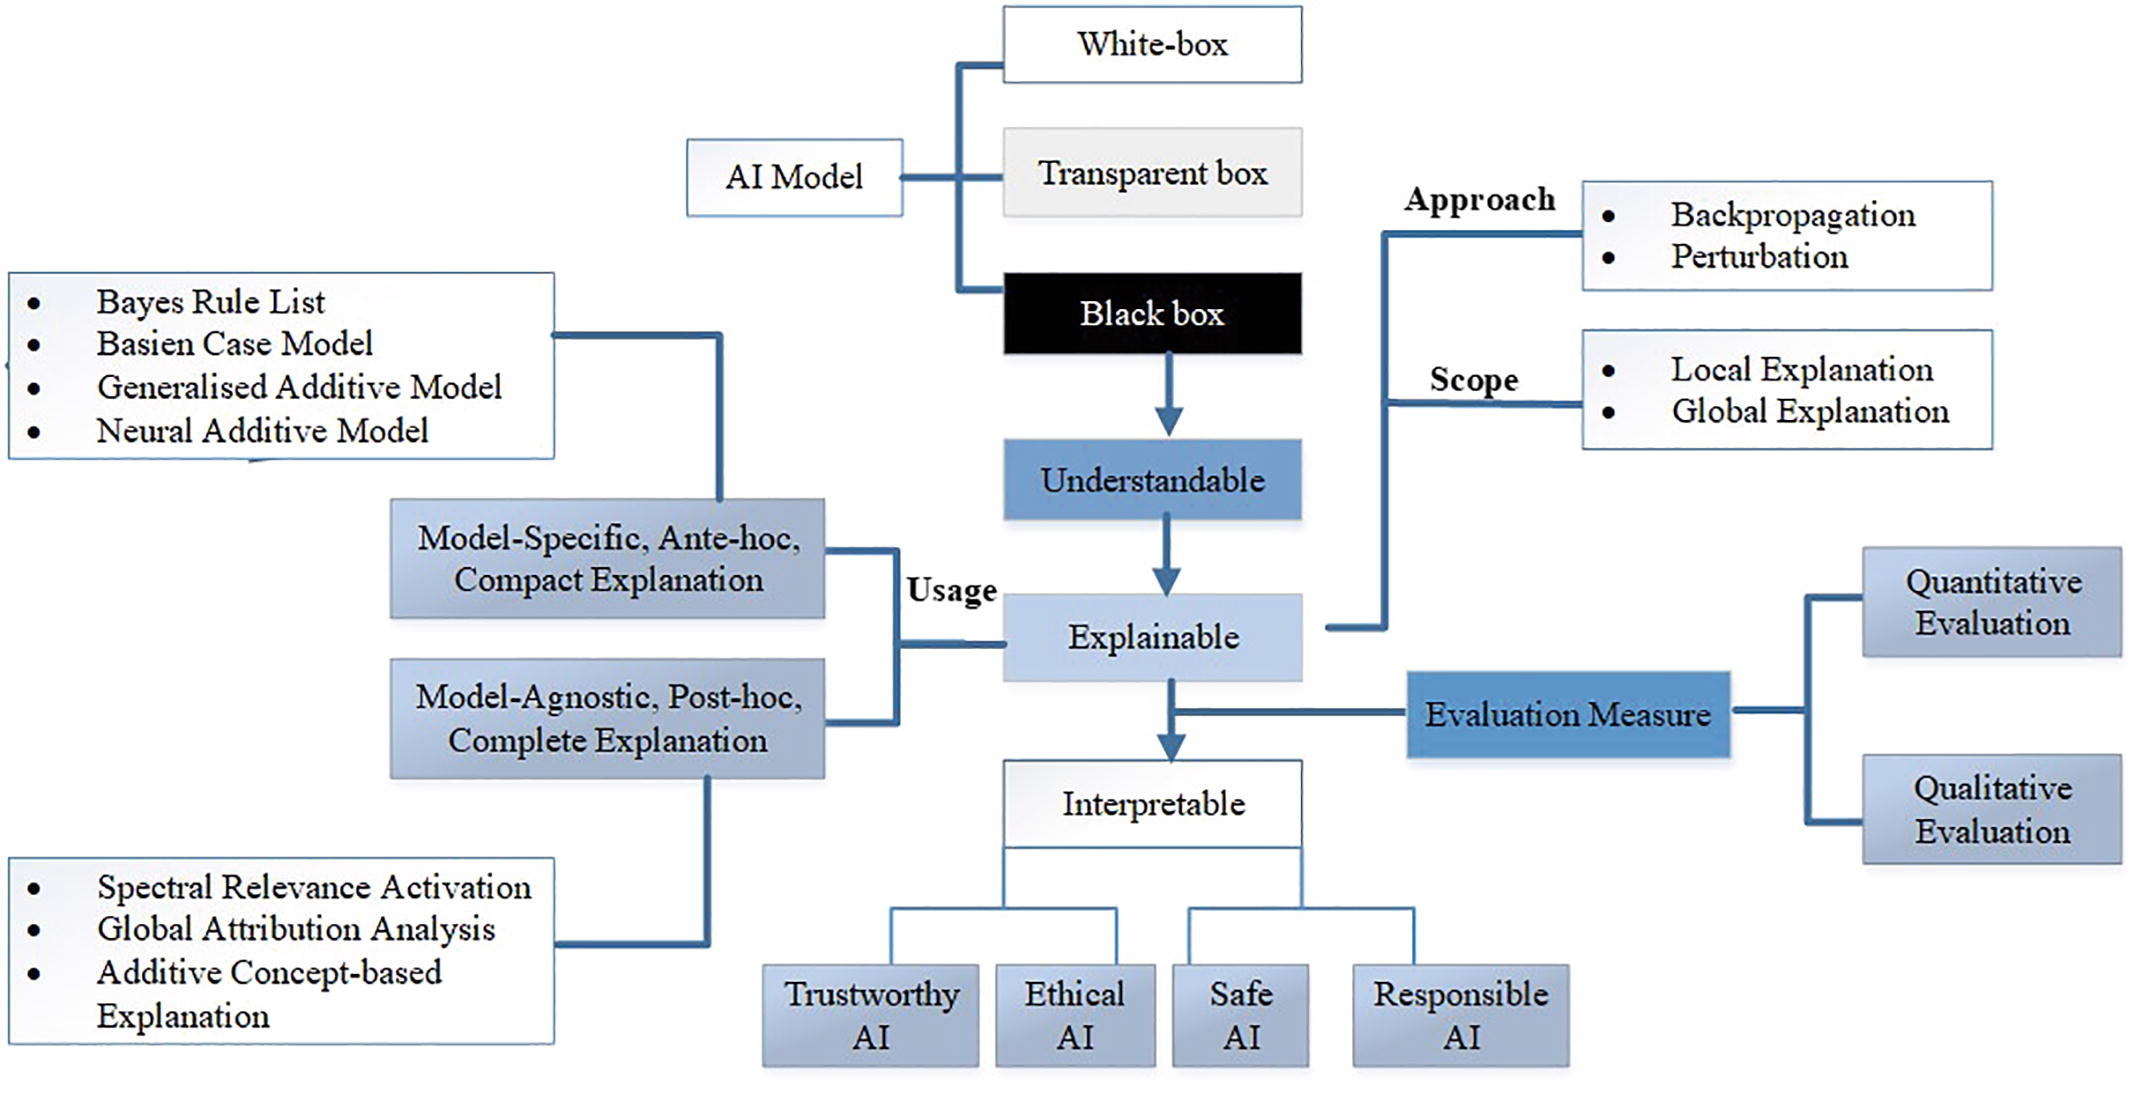
\includegraphics[width=1\textwidth]{images/CH02_algorithms_overview_Saleem.jpg}
    \caption{Explainability Overview, from \cite{SALEEM2022165}}
    \caption*{Overview of the concepts related to explainability algorithms.}
    \label{fig:Explainability_overview}
\end{figure}

The two most widely adapted local, model-agnostic, post-hoc methods are \textit{SHAP} (SHapley Additive exPlanations) \parencite{Lundberg2017} and \textit{LIME} (Local Interpretable Model-agnostic Explanations) \parencite{Ribeiro2016}.

\textbf{SHAP} is based upon the use of Shapley values used in coalitional game theory and aims to weight the importance of each feature to the result by game-theoretically distributing the value of the final prediction among all features being included \parencite{Molnar2023}.
The key features of SHAP are (based on \cite{Molnar2023})
\begin{itemize}
    \item \textbf{Additivity}: All feature contributions can be summed up in a linear way, benefitting understandability of the explanations.
    \item \textbf{Local Accuracy}: SHAP values are locally accurate, as predictions for a given input can be calculated as a result of the expected model output and the specific score for the local input.
    \item \textbf{Missingness}: As missingness in features is attributed zero values, missingness does not skew outcomes.
    \item \textbf{Consistency}: SHAP values do not change upon model change, but only when the actual feature contributions change.
\end{itemize}

\textbf{LIME} is based upon trying to approximate the model's decision boundary locally by perturbing the input data and observing the change in the model's output \parencite{Molnar2023}.

A way of globally assessing model explainability is the use of \textbf{(Global) Surrogate Models} (as opposed to e.g. the LIME algorithm, which can be considered a local surrogate model). 
These aim to make black-box algorithm decisions explainable by implementing white-box models to learn the decision criteria that the black-box model has established by being trained on the black-box predictions (compare e.g. \cite{Karim2023}).
Instead of making the predictions themselves explainable, these models aim to making the underlying decision criteria understandable \parencite{Molnar2023}.

\subsection{Explainability and Fairness}\label{subsec:Explainability_fairness}

%In order to conclude this literature review, this section will evaluate how the the concepts of fairness and explainability are related to each other, showing that the analysis of each adds separate value to this thesis.

Explainability and fairness within the field of Machine Learning do not inherently share the same scope. On the one hand, as an example, explainability is a rather objective concept, focusing on describing a model's inner workings neutrally. 
Comparing that to fairness it becomes apparent that the latter is a more subjective concept, as it is dependent on the context and man-made definitions, which are often rooted in certain (e.g.\ political) interpretations of fairness \parencite{Deepak2021}.
Yet, both concepts are somewhat dependent as assessing model fairness requires an understanding of the factors influencing a prediction \parencite{Zhou2022}.
Subsequently, approaches to connect both concepts have been proposed in academic literature. 
%Two different approaches are proposed by Deepak \parencite{Deepak2021}: 
%\begin{itemize}
%    \item \textbf{Interpretability for fairness (IFF)}: IFF is a framework intending to ensure that supposedly fair decisions made by AI are truly fair. The two steps in order to achieve that are \textit{clearly laying out the values supposed to adhered to} and \textit{explaining decisions made with regards to how they relate to those values}.
%    \item \textbf{Fairness and Interpretations (F\&I)}: F\&I is a multi-layered approach, which, in the first step, aims to satisfy both fairness and interpretability requirements based on given constraints. If both criteria in combination cannot satisfyingly be met, the user needs to be informed that the model is not sufficiently interpretable, but yet adheres to at least one of the two desired properties.
%\end{itemize}
However, these concepts are only stated on theoretical level without practical implications in this paper and are therefore not directly applicable for practitioners.


% Following Zhou's line of reasoning \parencite{Zhou2022}, other important approaches to merge the ideas of fairness and explainability in academic literature include:

% \textbf{Explanation as a way of guaranteeing fairness}: ... Papers!

% \textbf{Explanation as a way of shaping the perception of fairness}: ... Papers!

% \textbf{Perceived fairness of feature properties}: ... Papers!


Another promising approach to merge the concepts of fairness and explainability is the identification of root-causes for a certain model behavior by identifying \textit{influential subsets} within the underlying datasets as proposed by Pradhan \parencite{Pradhan2022}\footnote{For additional information on the proposed model see https://github.com/romilapradhan/gopher}.
By combining explainability criteria ('Why is a certain subgroup influential on the model's outcome?') with fairness criteria ('In how far can intervention in the training data regarding these subsets improve fairness?'), the authors manage to implement an efficient algorithm combining both concepts.

Just as it is the case for the aspect of fairness (as discussed in \textbf{chapter \ref{subsec:mortgage_lending_fairness}}), the field of mortgage lending has been specifically targeted by previous research on the aspect of explainability.
Maass et al. \parencite{Maass2022} contribute to the discussion by proposing the use of \textit{conceptual models} to capture the relationships in data, exemplarily using the HMDA 2020 dataset to predict mortgage approvals.
By using a total of 52 features clustered into different \textit{concepts} (i.e. abstracted groups of features), they determine the most important concepts relative to one another for the model's decision-making process.

In a comparative review of different explainability methods, Anderson evaluates the accuracy of explanations of different ML models on the 2019 HMDA dataset \parencite{Anderson2023}.
While all of the algorithms reviewed \textit{(most points lost, Shapley values, Shapley additive explanations, and the method of integrated gradients)} were able to provide explanations for the model's decisions, the accuracy of the explanations varied greatly between the different methods, with SHAP being the overall best-performing approach.

A very recent contribution to a research question from a similar field as this thesis has been made by Shiam et al. \parencite{Shiam2024}, who leverage explainable AI to assess the risk of credit default (as opposed to mortgage approval focused in this work), who leverage SHAP to explain predictions of a default classifier


%To-Do:
%Go through sources of Zhou and list important ones
%Mention specifically newly added analysis in this thesis
%Circle back to introduction: Why do both add value?

This thesis will add value to the discussion of fairness and explainability in Machine Learning by providing a novel approach to the analysis of both concepts in the field of mortgage lending: 
By using explainability algorithms and enrichment data, the analysis of fairness will be supported and iteratively adjusted with the aim of finding the optimal balance of both concepts.
\chapter{Data and Methodology}\label{ch:Data_and_Methodology}



\section{Data}\label{sec:Data}



\subsection{HMDA Data}\label{subsec:HMDA_Data}

% Follow structure from presentation Ana: From where, why, which steps etc. - probably add in appendix the code for the enrichment?

The underlying data for this analysis was obtained \textit{\href{https://ffiec.cfpb.gov/data-browser/data/2022?category=states}{via the HMDA Data Browser}}. \@

XXX UPDATE! XXX

The data was filtered to only include entries from California, as it is the largest state in the US and thus provides a high amount of data. 
The time frame was set to 2022, as it is the most recent year available (!!!!!!!!!!). No filter was applied to the financial institutions, as the analysis is not focused on the institutions themselves. 
The data was further filtered to only include entries for single-family homes, as these are the most common type of homes and therefore provide the most data.

The raw dataset resulting from these filters contains $XXX$ entries and $XXX$ features, with a total sum of loan applications amounting to $XXX$ USD.

\subsection{Enrichment Data}\label{subsec:Enrichment_Data}

% Follow structure from presentation Ana: From where, why, which steps etc. - probably add in appendix the code for the enrichment?

The enrichment data was obtained from the \textit{\href{https://www.ers.usda.gov/data-products/county-level-data-sets/}{USDA ERS page}}. All available reports were downloaded, specifically the following datasets:

\begin{itemize}
    \item \textbf{Poverty} (2021 latest)
    \item \textbf{Population} (2022 latest)
    \item \textbf{Unemployment, and Median Household Income} (annual average 2022 unemployment and 2021 median income latest)
    \item \textbf{Education} (2017–21, 5-year average latest).
\end{itemize}

In order to clean and reshape the data in a easily analyzable format, the following steps were taken\footnote{For all detail, see the corresponding cleaning notebook at !!! XXX !!!}:
All datasets were \textit{filtered} to only contain CA county-level data, not the aggregated values for the full state of California and, in case multiple years of analysis were available, to only include the newest datapoints. 
Where there were more features available than would be useful for the analysis, the datasets were \textit{reduced} to only include the most relevant features, being:

\begin{itemize}
    \item \textbf{Poverty:} Only the percentage of the population living in poverty (PCTPOVALL\_2021) was included
    \item \textbf{Population:} Only the total population (POP\_ESTIMATE\_2022) was included
    \item \textbf{Unemployment, and Median Household Income:} The unemployment rate (Unemployment\_rate\_2022) and the median household income (Median\_Household\_Income\_2021) were included
    \item \textbf{Education:} All relative values, i.e.\ percentages of adults with their corresponding highest degrees were included.
\end{itemize}

All datasets were \textit{pivoted} in order to use the attributes as feature names and \textit{indexed} by the FIPS code and the name of the respective county. After basic \textit{checks for completeness}, the feature columns were \textit{renamed} for clarity. Finally, all datasets were \textit{merged} into a single dataframe, which was then \textit{exported} as a pickle file for further use in the analysis.

% Reasoning!

The cleaned data are \textit{complete} in a way that there are values available for all features and for all of the 58 counties. Basic summary statistics can be found in \textbf{Table \ref{tab:enrichment_summary}}. Expectedly, there is a high correlation between some of the features, see \textbf{Figure \ref{fig:CH03_Enrichment_Correlation}}.

\begin{table}[h]
    \centering
    \begin{tabularx}{\textwidth}{llllll}
    \hline
     & \textbf{Count} & \textbf{Mean} & \textbf{Std} & \textbf{Min} & \textbf{Max} \\
    \hline
    College Degree (Perc.) & 58.00 & 33.19 & 5.77 & 17.89 & 44.23 \\
    \hline
    Bachelor Degree or Higher (Perc.) & 58.00 & 28.55 & 12.27 & 11.77 & 60.15 \\
    \hline
    High School Degree (Perc.) & 58.00 & 23.77 & 5.84 & 10.17 & 38.42 \\
    \hline
    Less than High School Degree (Perc.) & 58.00 & 14.49 & 7.02 & 4.87 & 29.65 \\
    \hline
    Population (thousands) & 58.00 & 672.92 & 1,428.89 & 1.19 & 9,721.14 \\
    \hline
    Poverty Rate (Perc.) & 58.00 & 13.63 & 3.96 & 6.60 & 21.90 \\
    \hline
    Median Household Income (thousands) & 58.00 & 75.30 & 21.89 & 45.51 & 141.16 \\
    \hline
    Unemployment Rate (Perc.) & 58.00 & 4.84 & 2.07 & 2.40 & 14.70 \\
    \hline
    \end{tabularx}
    \caption{Summary Statistics of the Enrichment Data}
    \label{tab:enrichment_summary}
\end{table}

\begin{figure}[h]
    \centering
    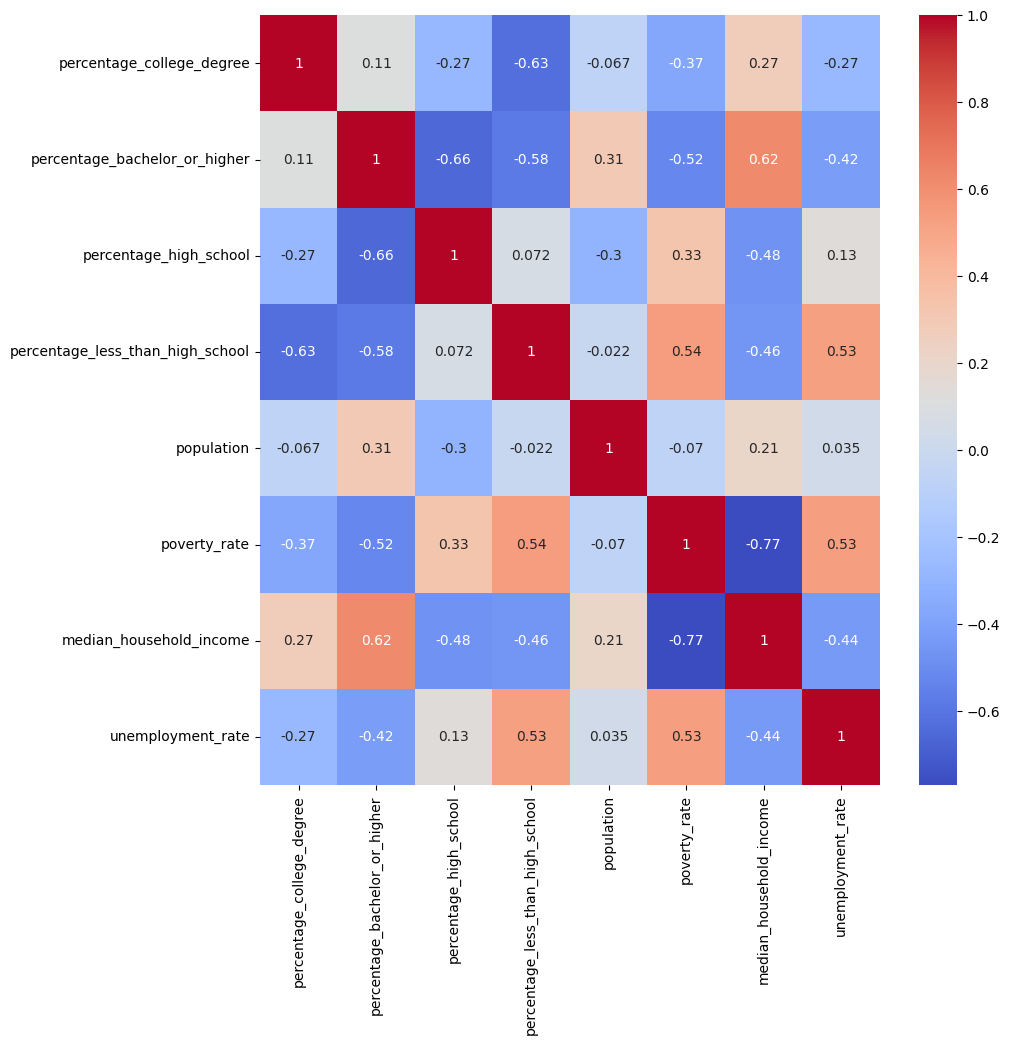
\includegraphics[width=0.7\textwidth]{images/CH03_Enrichment_Correlation.png}
    \caption{Correlation Between the Enrichment Features}
    \label{fig:CH03_Enrichment_Correlation}
\end{figure}

\section{Methodology}\label{sec:Methodology}
\chapter{Results}\label{chap:Results}

\section{Exploratory Data Analysis}\label{sec:Exploratory_Data_Analysis}

\subsection{HMDA Data}\label{subsec:HMDA_EDA}

After all preparation steps detailed in \textbf{chapter \ref{subsec:HMDA_Data}}, the dataset contained \textit{851,936} observations and \textit{9} features (including the target variable, \textit{loan\_granted}). 

\textbf{EDA of the Target Variable}

The target variable, \textit{loan\_granted}, is binary (\textit{Granted} or \textit{Not Granted}) and slightly imbalanced, with \textit{57.9\%} of all loans being granted. 
There were no missing values. The distribution of the target variable can be seen in \textbf{figure \ref{fig:CHXX_Target_Variable_Distribution}}.

\begin{figure}[!htbp]
    \centering
    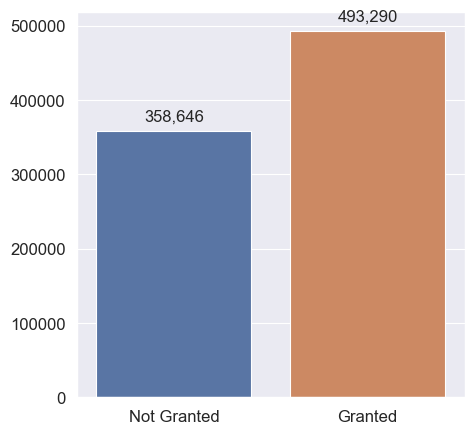
\includegraphics[width=0.6\textwidth]{images/CHXX_Target_Variable_Distribution.png}
%    \caption{HMDA: Distribution of the Target Variable}
%    \medskip
%    \small
%    The target variable is slightly imbalanced, with 57.9\% (493,290) of all loans being granted.
    \caption[HMDA: Distribution of the Target Variable]{\textbf{HMDA: Distribution of the Target Variable} - The target variable is slightly imbalanced, with 57.9\% (493,290) of all loans being granted.}
    \label{fig:CHXX_Target_Variable_Distribution}
\end{figure}

Analyzing the correlation of the target variable with the categorical and numerical features showed that the \textit{debt\_to\_income\_ratio} feature has the highest correlation (moderate negative correlation of \textbf{-0.61}) with the target variable, while the other features show only weak correlations. 
The correlation of the target variable with the numerical and categorical features was calculated by pairwise Pearson correlation, with the categorical features being encoded as integers before the calculation.
The results can be seen in \textbf{table \ref{tab:CHXX_Target_Correlation_Categorical}} and \textbf{figure \ref{fig:CHXX_Target_Correlation_Numerical}}, respectively.

%\begin{figure}[hbt!]
%    \centering
%    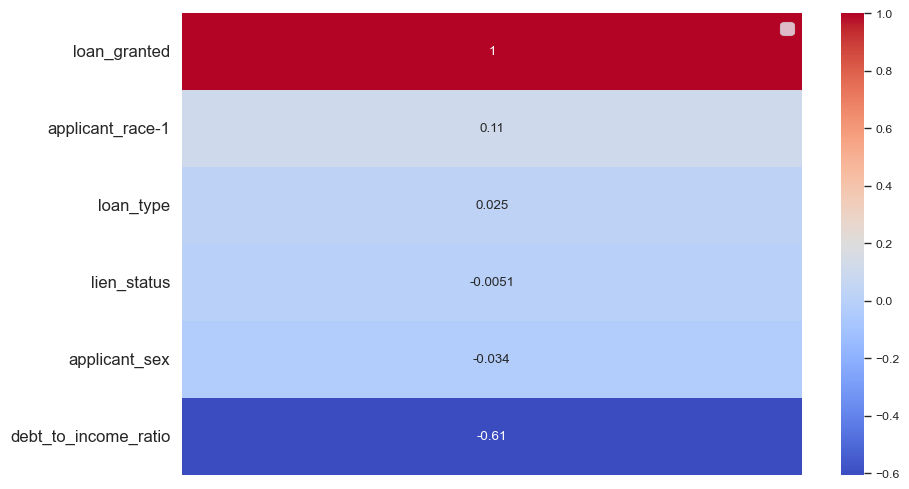
\includegraphics[width=1\textwidth]{images/CHXX_Target_Correlation_Categorical.png}
%    \caption{HMDA: Correlation of the Target Variable with Categorical Features}
%    \medskip
%    \small
%    While there are only weak correlations between \textit{loan\_granted} and \textit{applicant\_race-1, loan\_type, lien\_status}, and \textit{applicant\_sex}, there is a moderate negative correlation of \textbf{-0.61} between \textit{loan\_granted} and \textit{debt\_to\_income\_ratio}.
%    \label{fig:CHXX_Target_Correlation_Categorical}
%\end{figure}

\begin{table}[!htbp]
    \centering
    \begin{tabular}{l c}
    \toprule
    \textbf{Feature} & \textbf{Correlation Coefficient} \\
    \midrule
    \textbf{Race} & 0.11 \\
    \textbf{Loan Type} & 0.025 \\
    \textbf{Lien Status} & -0.0051 \\
    \textbf{Sex} & -0.034 \\
    \textbf{Debt to Income Ratio} & -0.61 \\
    \bottomrule
    \end{tabular}
    \medskip
    \caption[HMDA: Correlation of the Target Variable with Categorical Features]{\textbf{HMDA: Correlation of the Target Variable with Categorical Features} - While there are only weak correlations between \textit{granted loans} and \textit{applicant race, lien status, loan type}, and \textit{applicant sex}, there is a moderate negative correlation of \textbf{-0.61} between \textit{granted loans} and \textit{debt to income ratio}.}
    \label{tab:CHXX_Target_Correlation_Categorical}
\end{table}

\begin{figure}[!htbp]
    \centering
    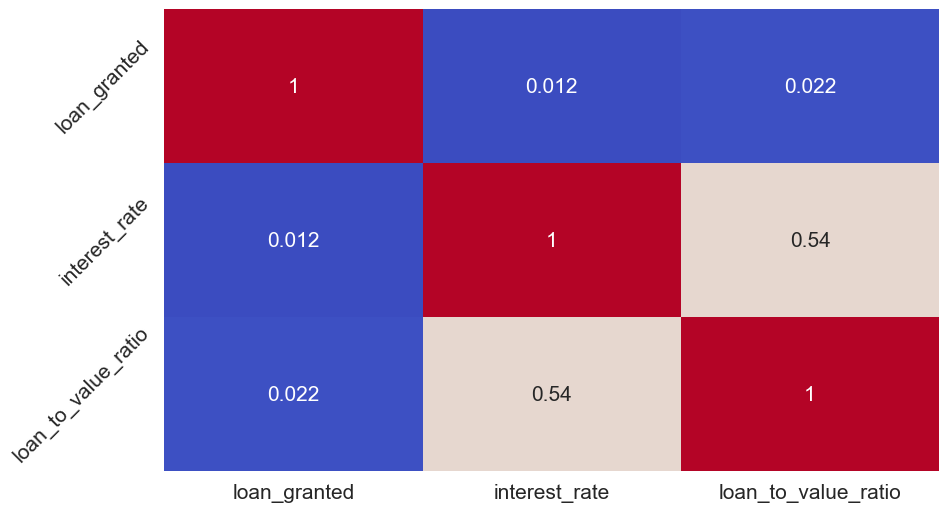
\includegraphics[width=0.8\textwidth]{images/CHXX_Target_Correlation_Numerical.png}
%    \caption{HMDA: Correlation Between the Numerical Features}
%    \medskip
%    \small
%    While both numerical features are only weakly correlated with \textit{loan\_granted}, there is a moderate positive correlation of \textbf{0.54} inbetween them.
    \caption[HMDA: Correlation Between the Numerical Features]{\textbf{HMDA: Correlation Between the Numerical Features} - While both numerical features are only weakly correlated with \textit{loan\_granted}, there is a moderate positive correlation of \textbf{0.54} inbetween them.}
    \label{fig:CHXX_Target_Correlation_Numerical}
\end{figure}

% \subsection{Data Overview}\label{subsec:Data_Overview}

\textbf{EDA of the Features}

The processed dataset contained two \textit{numerical} features: \textbf{interest\_rate} and \textbf{loan\_to\_value\_ratio}.
% Their distributions can be seen in \textbf{Figure \ref{fig:CHXX_Numerical_Distributions_1}} and \textbf{Figure \ref{fig:CHXX_Numerical_Distributions_2}}.
Their distributions can be seen in \textbf{figure \ref{fig:CHXX_Numerical_Distributions_2}}.
% Both are positively correlated with each other with a correlation coefficient of \textit{0.54}.

%\begin{figure}[h]
%    \centering
%    \caption{Boxplots of the Numerical Features}
%    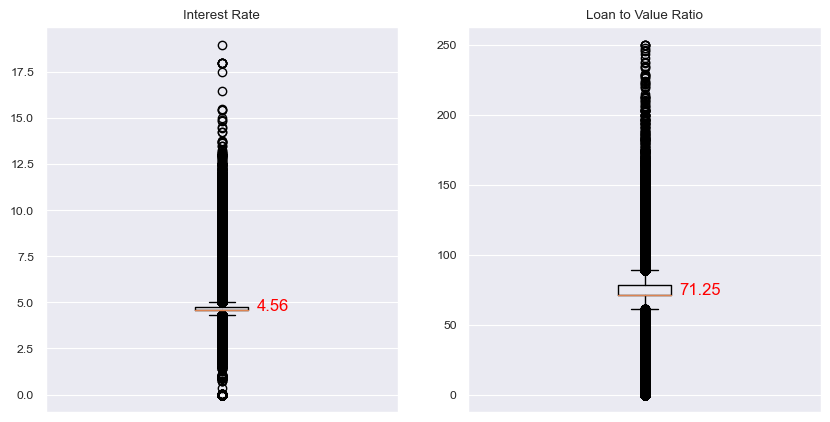
\includegraphics[width=0.85\textwidth]{CHXX_Numerical_Distributions_1.png}
%    \caption*{The results of the KNNImputer applying mean (annotated in red) values for all missing values show clearly here by the narrow quartiles.}
%    \label{fig:CHXX_Numerical_Distributions_1}
%\end{figure}

\begin{figure}[!htbp]
    \centering
    \begin{minipage}{0.5\textwidth}
        \centering
        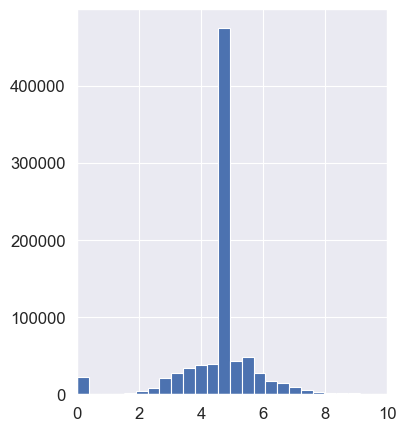
\includegraphics[width=\textwidth]{images/CHXX_Numerical_Distributions_2_IR.png}
        \small
        Interest Rate
    \end{minipage}\hfill
    \begin{minipage}{0.5\textwidth}
        \centering
        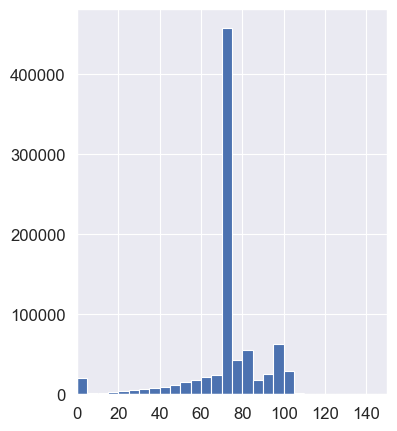
\includegraphics[width=\textwidth]{images/CHXX_Numerical_Distributions_2_LTVR.png}
        \small
        Loan to Value Ratio
    \end{minipage}    
%    \caption{HMDA: Histograms of the Numerical Features}
%    \medskip
%    \small
%    The results of the KNNImputer applying mean (\textit{4.56\%} for the interest rate and \textit{71.24\%} for the Loan to Value Ratio) values for the loan to value ratio values for all missing values show clearly here by the high amount of values at the mean.
    \caption[HMDA: Histograms of the Numerical Features]{\textbf{HMDA: Histograms of the Numerical Features} - The results of the KNNImputer applying mean (\textit{4.56\%} for the interest rate and \textit{71.24\%} for the Loan to Value Ratio) values for the loan to value ratio values for all missing values show clearly here by the high amount of values at the mean.}
    \label{fig:CHXX_Numerical_Distributions_2}
\end{figure}

Exploratory data analysis of the categorical variables showed that the majority of loan applicants are \textbf{White} (65\%) and \textbf{Male} (85\%), resulting in 57\% of all applicants being both White and Male.
Most loans applied for are \textbf{Conventional} (82\%) and \textbf{First Lien} (86\%).
Aside from missingness in the \textit{debt\_to\_income\_ratio} feature, which alone accounts for 26\% of all values, the data in this feature are roughly normally distributed, with the mode being 14\% of values in the \textbf{36\%-41\%} range. 
The distributions of the categorical variables can be seen in \textbf{figure \ref{fig:HMDA_Categorical_Features_Distributions}}.

\begin{figure}[!htbp]

    \centering

    \begin{minipage}[b]{0.5\textwidth}
        \centering
        \begin{subfigure}[t]{0.06\textwidth}
            \textbf{a)}
        \end{subfigure}
        \begin{subfigure}[t]{0.9\textwidth}
            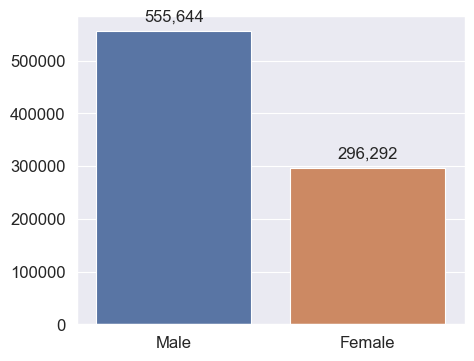
\includegraphics[width=\linewidth, valign=t]{images/HMDA_features/HMDA_features_sex.png}
        \end{subfigure}
    \end{minipage}%
    \begin{minipage}[b]{0.5\textwidth}
        \centering
        \begin{subfigure}[t]{0.06\textwidth}
            \textbf{b)}
        \end{subfigure}
        \begin{subfigure}[t]{0.9\textwidth}
            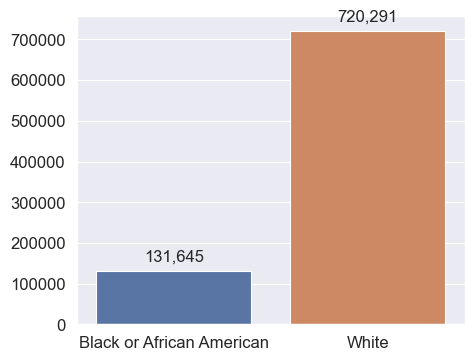
\includegraphics[width=\linewidth, valign=t]{images/HMDA_features/HMDA_features_race.png}
        \end{subfigure}
    \end{minipage}%
    \hfill\allowbreak%
    \begin{minipage}[b]{0.5\textwidth}
        \centering
        \begin{subfigure}[t]{0.06\textwidth}
            \textbf{c)}
        \end{subfigure}
        \begin{subfigure}[t]{0.9\textwidth}
            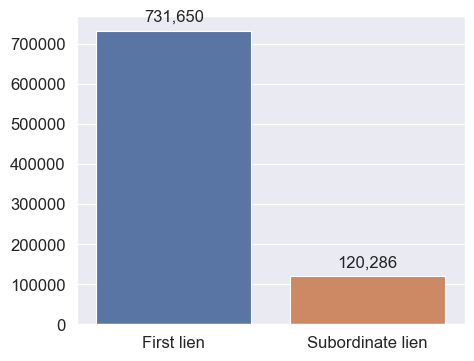
\includegraphics[width=\linewidth, valign=t]{images/HMDA_features/HMDA_features_lien.png}
        \end{subfigure}
    \end{minipage}%
    \begin{minipage}[b]{0.5\textwidth}
        \centering
        \begin{subfigure}[t]{0.06\textwidth}
            \textbf{d)}
        \end{subfigure}
        \begin{subfigure}[t]{0.9\textwidth}
            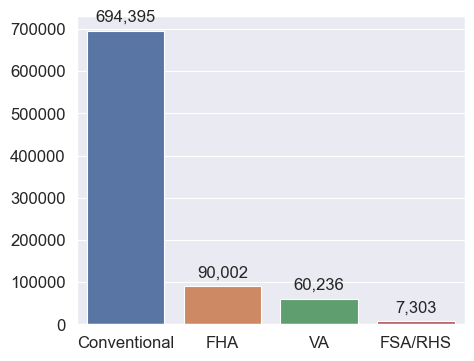
\includegraphics[width=\linewidth, valign=t]{images/HMDA_features/HMDA_features_type.png}
        \end{subfigure}
    \end{minipage}%
    \hfill\allowbreak%
    \begin{minipage}[b]{1\textwidth}
        \centering
        \begin{subfigure}[t]{0.06\textwidth}
            \textbf{e)}
        \end{subfigure}
        \begin{subfigure}[t]{0.92\textwidth}
            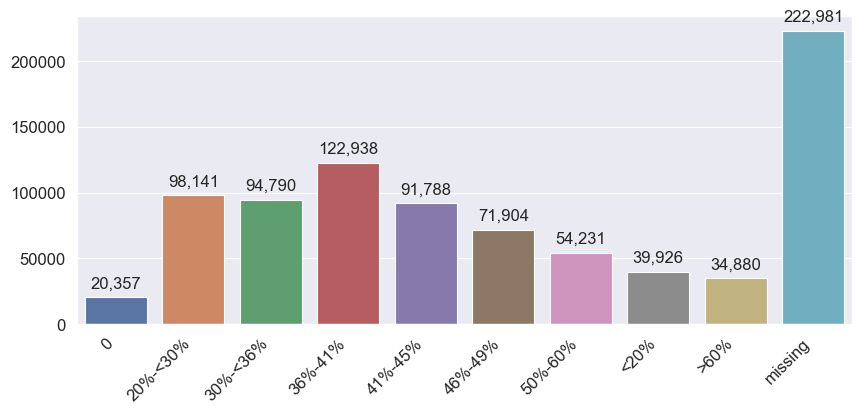
\includegraphics[width=\linewidth, valign=t]{images/HMDA_features/HMDA_features_dtir.png}
        \end{subfigure}
    \end{minipage}%

    \caption[HMDA: Distributions of the Categorical Features]{\textbf{HMDA: Distributions of the Categorical Features} - The majority of loan applicants are \textit{Male} and \textit{White} (see a) and b)). 
    Most loans applied for are \textit{Conventional} and \textit{First Lien} (see c) and d)). The \textit{debt\_to\_income\_ratio} feature is (apart from the missing values) roughly normally distributed, with the mode being 14\% of values in the \textbf{36\%-41\%} range (see e)).}
    \label{fig:HMDA_Categorical_Features_Distributions}

\end{figure}

% \subsection{Fairness}\label{subsec:Fairness}

\textbf{EDA of Fairness Aspects}

Following the scope of this thesis specified in \textbf{chapter \ref{ch:Introduction}}, a special focus needs to be put  on fairness, specifically equality with regards to the protected attribute(s).
This potential unfairness in the underlying data can be identified from assessing the distribution of the target variable across different groups.
\textbf{Figure \ref{fig:CHXX_Loan_Grant_By_Protected_Attribute}} shows the amount of (not) granted loans per race and by sex, the probabilities of being granted a loan across these groups can be found in \textbf{table \ref{tab:loan_granting}}.\@

\begin{figure}[!htbp]
    \centering
    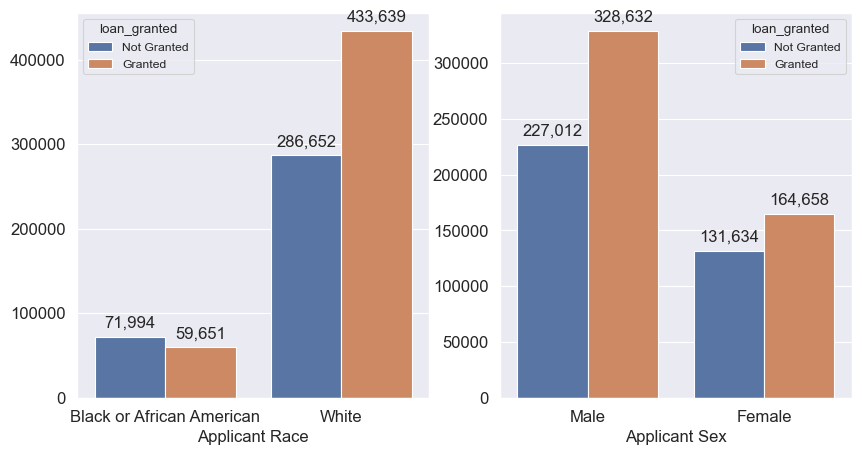
\includegraphics[width=0.85\textwidth]{images/CHXX_Loan_Grant_By_Protected_Attribute.png}
%    \caption{Loan Grant by Protected Attribute}
%    \caption*{Discrimination by race is apparent in the data, as the amount of granted loans differs significantly}
%    \medskip
    \caption[Loan Grant by Protected Attribute]{\textbf{Loan Grant by Protected Attribute} - Discrimination by race is apparent in the data, as the amount of granted loans differs significantly.}
    \label{fig:CHXX_Loan_Grant_By_Protected_Attribute}
\end{figure}

\begin{table}[!htbp]
    \centering
      \begin{tabular}{lcc}
      \toprule
      \textbf{Applicant Race} & \textbf{Applicant Sex} & \textbf{Loan Granted (\%)} \\
      \midrule
      Black or African American & Male    & 46.4 \\
            & Female  & 44.1 \\
      White & Male    & 60.9 \\
            & Female  & 58.8 \\
      \bottomrule
      \end{tabular}
%      \caption{Loan Granting Statistics by Applicant Race and Sex}
%      \caption*{Analyzing the differences in percentages of loans being granted among race and sex of applicants shows differences in the underlying data: Regardless of their gender, Black or African American applicants are less likely to be granted a loan than White applicants.}
    \medskip
    \caption[Loan Granting Statistics by Applicant Race and Sex]{\textbf{Loan Granting Statistics by Applicant Race and Sex} - Analyzing the differences in percentages of loans being granted among race and sex of applicants shows differences in the underlying data: Regardless of their gender, Black or African American applicants are less likely to be granted a loan than White applicants.}
    \label{tab:loan_granting}%
\end{table}%

Even though the focus of the analysis is on the \textit{applicant\_race-1} attribute, \textit{applicant\_sex} has been included as a second discriminating factor, as it also constitutes a protected attribute.
Inspection of the results depicted here did however imply that the issue of racial equality is more pronounced than that of inequality between the sexes.
A chi-squared test of independence proved that assumption of underlying inequality between races in the data, as the p-value is \textit{<0.01} and therefore H0 (equality in granted loans) could be rejected at any significance level.
Using the aforementioned \textbf{AIF360} package to assess the mean difference of granted loans between the races in the underlying data amounted to a \textit{14.9\%} difference.

\subsection{Enrichment Data}\label{subsec:Enrichment_Data}

The cleaned enrichment data (see \textbf{chapter \ref{subsec:Enrichment_Data}}) are \textit{complete} in a way that there are values available for all features and for all of the 469 counties. Basic summary statistics can be found in \textbf{table \ref{tab:enrichment_summary}}. 
Across all 469 counties that are included in this analysis, a high school degree is the most common highest degree, with the mean of population percentages with that degree being \textbf{32.9\%} overall, followed by a college degree with \textbf{30.9\%}. 
A high discrepancy in the educational standard between the different observational units becomes apparent when considering the presence of counties where \textbf{81.6\%} of the population have less than a high school degree, while in others, \textbf{55.2\%} have a bachelors degree or higher.
In terms of population, the counties in this analysis are heterogenous as well, with the mean population being \textbf{85.36 thousand} with standard deviation of \textbf{318.70 thousand} and the most inhabited county having nearly 100,000 times as many inhabitants as the least inhabited.
The socio-economic factors expose a wide range of values as well, with the poverty rate ranging from \textbf{3.9\%} to \textbf{43.5\%}, the median household income from \textbf{25.65 thousand} to \textbf{124.35 thousand}, and the unemployment rate from \textbf{0.6\%} to \textbf{11.0\%}.

\begin{table}[!htbp]
    \centering
    \begin{tabularx}{\textwidth}{l *{5}{>{\centering\arraybackslash}X}}
    \hline
     & \textbf{Count} & \textbf{Mean} & \textbf{Std} & \textbf{Min} & \textbf{Max} \\
    \hline
    College Degree & 469.00 & 30.9\% & 6.03 & 0.00\% & 76.92\% \\
    Bachelor Degree or Higher & 469.00 & 21.7\% & 8.42 & 0.00\% & 55.17\% \\
    High School Degree & 469.00 & 32.9\% & 6.60 & 12.93\% & 51.17\% \\
    Less than High School Degree & 469.00 & 14.5\% & 8.18 & 0.60\% & 81.55\% \\
    Population (thousands) & 469.00 & 85.36 & 318.70 & 0.05 & 4,780.91 \\
    Poverty Rate & 469.00 & 15.9\% & 6.23 & 3.90\% & 43.50\% \\
    Median Household Income (thousands) & 469.00 & 56.6 & 13.94 & 25.65 & 124.35 \\
    Unemployment Rate & 469.00 & 3.6\% & 1.21 & 0.60\% & 11.00\% \\
    \hline
    \end{tabularx}
%    \caption{Summary Statistics of the Enrichment Data}
%    \small
%    The summary statistics show that the data is complete and has a wide range of values.
    \medskip
    \caption[Summary Statistics of the Enrichment Data]{\textbf{Summary Statistics of the Enrichment Data} - The summary statistics show that the data is complete and has a wide range of values.}
    \label{tab:enrichment_summary}
\end{table}

%A closer look into the discrepancies between the highest and lowest values of selected enrichment features can be found in \textbf{figure \ref{fig:CH03_Geo_High_Low}}.
%In terms of population, the high discrepancy betwen lowest and highest value is pronounced by the fact that the highest populated \textit{Harris County} has nearly twice as many inhabitants as the second-largest \textit{Dallas County}, while the lowest populated \textit{Loving County} has less than a fourthof the inhabitants of the second-smallest \textit{King County}.
%Similar outlier values can be found in the unemployment rate with \textit{Loving county} (0.6\%) differing strongly from 

%\begin{figure}[h]
%    \centering
%    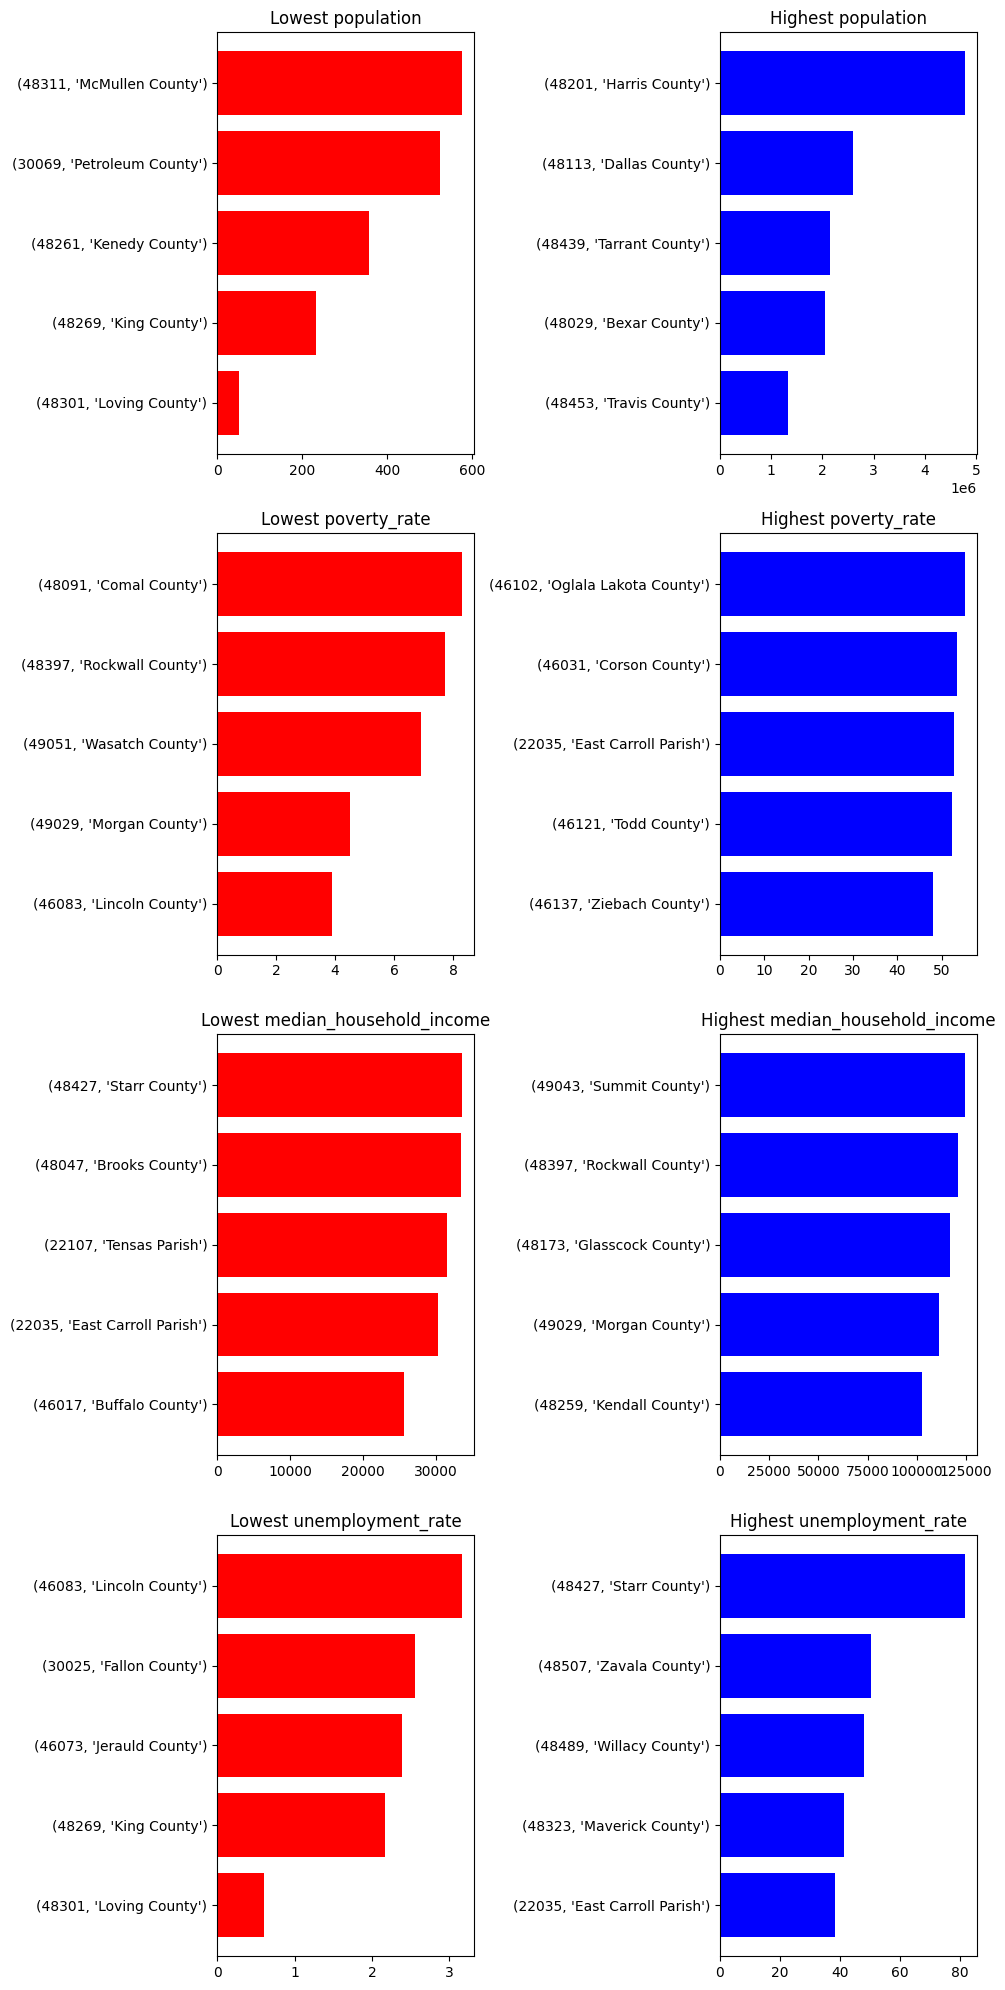
\includegraphics[width=0.85\textwidth]{images/CH03_Geographic_Low_vs_High.png}
%    \caption{Highest and Lowest Values of Selected Enrichment Features}
%    \medskip
%    \small
%    There is a wide range in the numerical enrichment features, creating some natural outliers.
%    \label{fig:CH03_Geo_High_Low}
%\end{figure}

Expectedly, there is a high correlation between some of the features (see \textbf{figure \ref{fig:CH03_Enrichment_Correlation}}).
While a bachelors degree or higher tends to be associated with a higher median household income (positive correlation of \textbf{0.62}), a high school degree or less than a high school degree as a highest degree is associated with a higher poverty rate (positive correlation of \textbf{0.33} and \textbf{0.54} respectively).
A similar relation of socio-economic factors with education can be observed in the correlation of the unemployment rate with the highest degree, with a negative correlation of \textbf{-0.42} for holders of a bachelors degree or higher, compared to a positive correlation of \textbf{0.53} for less than a high school degree, implying that on average, observational units with less than a high school degree a more likely to be unemployed than those with a bachelors degree or higher.

\begin{figure}[h]
    \centering
    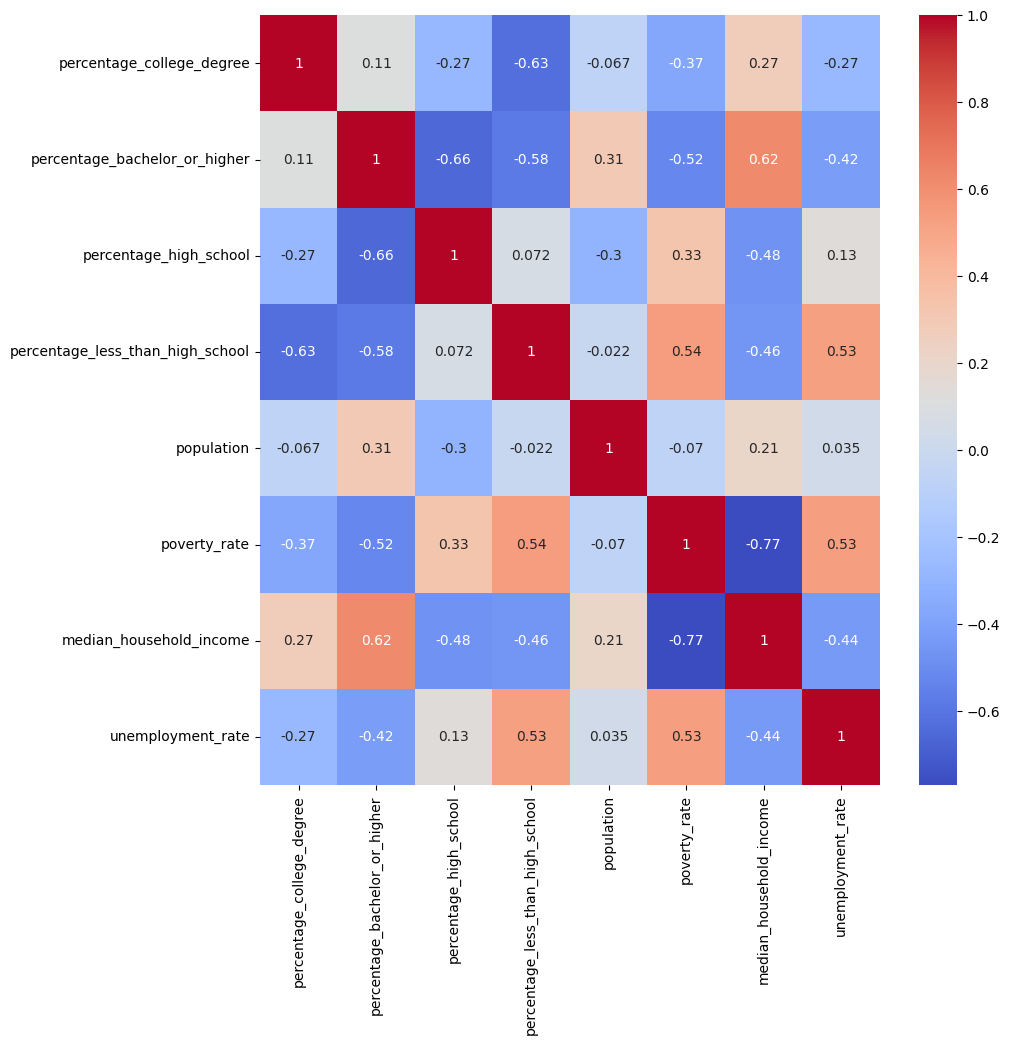
\includegraphics[width=0.85\textwidth]{images/CH03_Enrichment_Correlation.png}
%    \caption{Correlation Between the Enrichment Features}
%    \medskip
%    \small
%    Some of the enrichment features expectedly show a high correlation, an example being \textit{median\_household\_income} and \textit{poverty\_rate}.
    \caption[Correlation Between the Enrichment Features]{\textbf{Correlation Between the Enrichment Features} - Some of the enrichment features expectedly show a high correlation, an example being \textit{median\_household\_income} and \textit{poverty\_rate}.}
    \label{fig:CH03_Enrichment_Correlation}
\end{figure}

As stated before, analyzing the geographical information provided in the enrichment dataset (see \textbf{chapter \ref{subsec:Explainability}}) was expected to provide additional insights into the fairness of the model.
A sign of potential discrimination in the data could be the correlation between race and potentially favorable outcomes, such as a higher percentage of granted loans or a lower poverty rate.
\textbf{Figure \ref{fig:Scatter_White_Applicants_Loan_Grant}} shows a scatterplot that relates the percentage of White applicants to the percentage of granted loans per county. It indicates that a higher percentage of white applicants per county does not only seem to be correlated with a higher percentage of these loans actually being granted, but also with a lower poverty rate on average.

\begin{figure}[!htbp]
    \centering
    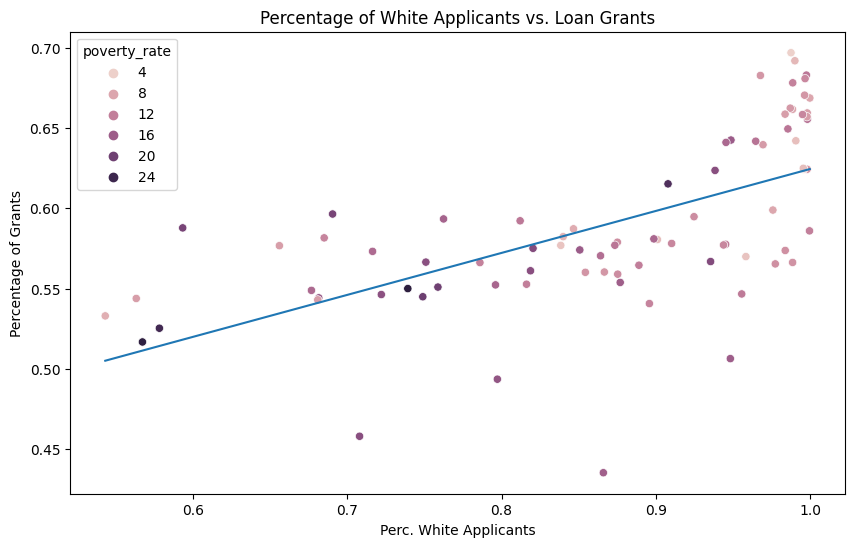
\includegraphics[width=0.85\textwidth]{images/CHXX_Perc_Grants_vs_Perc_White.png}
%    \caption{Relationship between Applicant Race, Poverty Rate and Loan Grants}
%    \caption*{Counties with predominantly White applicants do not only tend to have a lower poverty rate on average, but also see a higher percentage of loans being granted on average.}
    \caption[Relationship between Applicant Race, Poverty Rate and Loan Grants]{\textbf{Relationship between Applicant Race, Poverty Rate and Loan Grants} - Counties with predominantly White applicants do not only tend to have a lower poverty rate on average, but also see a higher percentage of loans being granted on average.}
    \label{fig:Scatter_White_Applicants_Loan_Grant}
\end{figure}

It should be noted that the distributions within the enrichment data themselves are skewed by nature, as there are way higher numbers of White applicants in the data set and only few counties have a substantial number of predicted mortgage grants (see \textbf{figure \ref{fig:Enrichment_Data_EDA}}).

\begin{figure}[!htbp]
    \centering
    \begin{minipage}{0.33\textwidth}
        \centering
        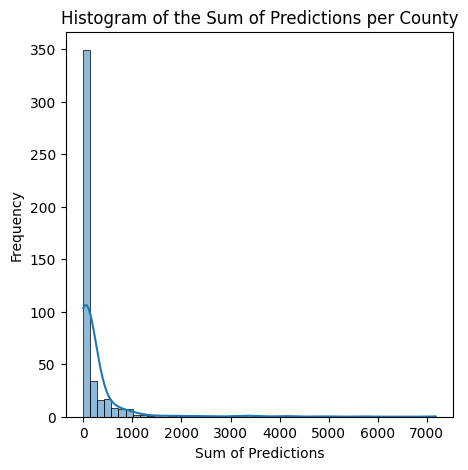
\includegraphics[width=\textwidth]{images/geo_enrich/predictions_per_county.png}
        \small
        Applications per County
    \end{minipage}\hfill
    \begin{minipage}{0.33\textwidth}
        \centering
        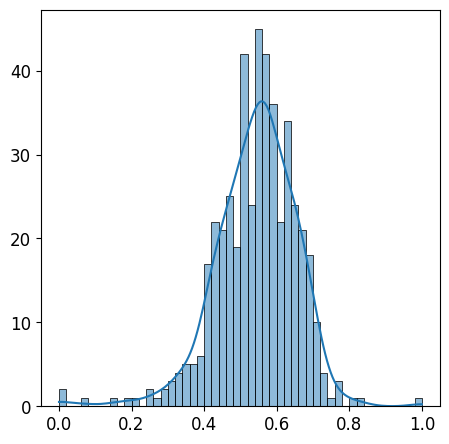
\includegraphics[width=\textwidth]{images/geo_enrich/perc_predictions.png}
        \small
        Percentage of Grants
    \end{minipage}\hfill
    \begin{minipage}{0.33\textwidth}
        \centering
        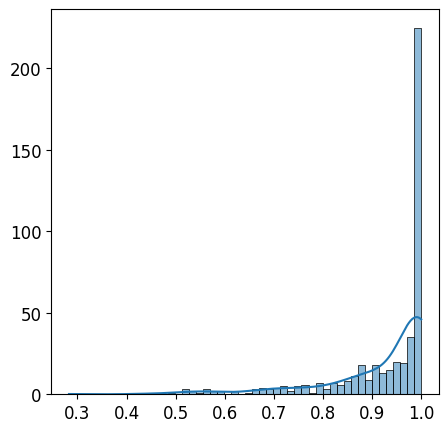
\includegraphics[width=\textwidth]{images/geo_enrich/white_per_county.png}
        \small
        Percentage of White Applicants
    \end{minipage}\hfill
%    \caption{Enrichment Data EDA}
    \caption[Enrichment Data EDA]{\textbf{Enrichment Data EDA} - Analyzing the enrichment data shows that while the percentage of predictions per county appears to be normally distributed, the distributions of the percentage of White applicants and the percentage of predicted loans per county are skewed.}
    \label{fig:Enrichment_Data_EDA}
%    \medskip
%    \small
%    Analyzing the enrichment data shows that while the percentage of predictions per county appears to be normally distributed, the distributions of the percentage of White applicants and the percentage of predicted granted loans per county are skewed.
\end{figure}

\newpage

%\section{Results}\label{sec:Results}      

As defined in \textbf{chapter \ref{subsec:Performance_Assessment}} and \textbf{chapter \ref{subsec:Fairness_Assessment}}, each outcome is assessed in terms of performance and fairness with two pre-defined metric sets. Additionally, the aspect of Explainability will be demonstrated examplarily for the initial model run.

\subsection{Initial Performance}\label{subsec:Initial_Performance}

The initial run serving as a benchmark was conducted training the neural network described in \textbf{chapter \ref{subsec:Model_Training_and_Prediction}} on the unadjusted training data (see \textbf{chapter \ref{subsec:HMDA_Data}}).

\textbf{Explainability}

As was intended in \textbf{chapter \ref{subsec:Explainability}}, three different Explainability algorithms were utilized to challenge each other's results and analyze overall patterns. \textbf{figure \ref{fig:SHAP_explanations}} and \textbf{figure \ref{fig:LIME_explanations}} show the individual explanations for the first 150 observations of the test set provided by SHAP and LIME, respectively. 
As already mentioned in \textbf{chapter \ref{subsec:Performance_Assessment}}, the model behaved somewhat different from the expectations: Imputation of missing values in the \textit{debt\_to\_income\_ratio} feature led to a significant decrease in both fairness and performance measures of the model.
Therefore, it must be assumed that missingness in itself is not completely at random and holds information (or that the imputation method via a random forest regressor is not suitable for this task).
While SHAP considers that missingness to be the most important influence on model predictions, LIME weighs the \textit{debt\_to\_income\_ratio} features higher in general.
None of the algorithms consider the protected attributes to be of high direct impact on the results.

\begin{figure}[h]
    \centering
    \begin{minipage}{0.5\textwidth}
        \centering
        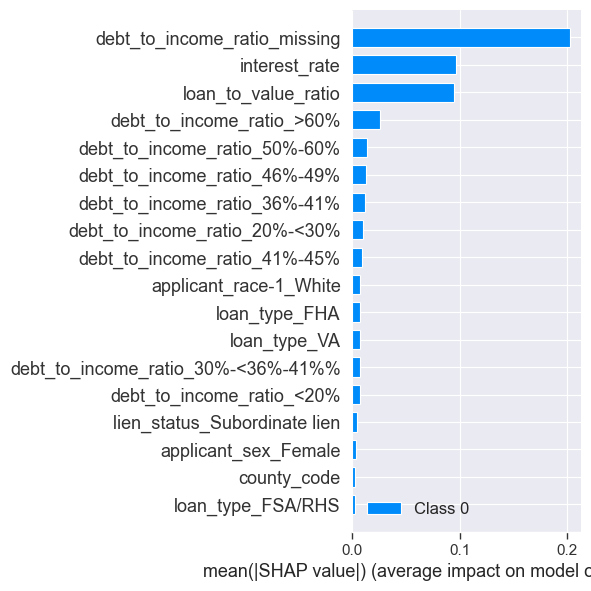
\includegraphics[width=\textwidth,height=5cm,keepaspectratio]{images/CHXX_UPDATE_SHAP_individual.png}
        \caption{SHAP individual explanations}
        \label{fig:SHAP_explanations}
    \end{minipage}\hfill
    \begin{minipage}{0.5\textwidth}
        \centering
        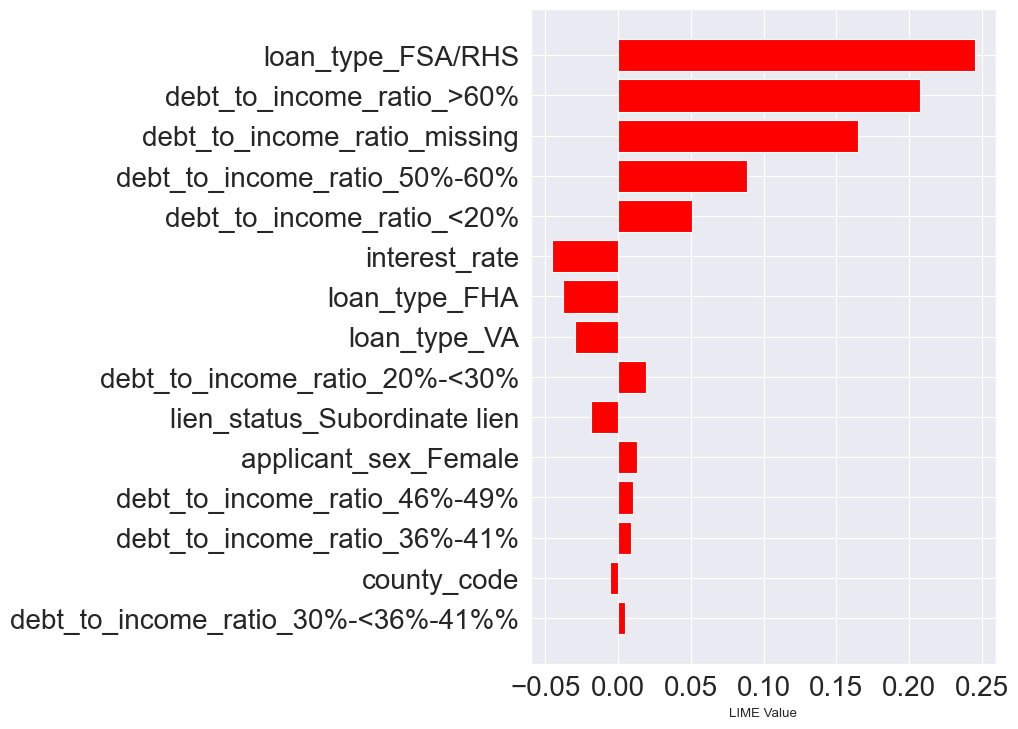
\includegraphics[width=\textwidth,height=5cm,keepaspectratio]{images/CHXX_UPDATE_LIME_individual.png}
        \caption{LIME individual explanations}
        \label{fig:LIME_explanations}
    \end{minipage}
    \caption*{Directly comparing LIME and SHAP explanations for the first 150 observations of the test set: While \textit{debt\_to\_income\_ratio} is an important factor in both explanations, its actual impact varies, as LIME also considers the \textit{loan\_type} feature to be of high importance. Default plotting options were kept: SHAP values are displayed as absolutes, while LIME values show the direction of their impact.}
\end{figure}

While the overall trends are similar with both algorithms, the actual impact of the features varies significantly. While this is not a direct threat to the quality of the results of this thesis, it is a reminder that Explainability algorithms need to be analyzed carefully. 
This ties with the findings of Krishna et al. \parencite{Krishna2022}, who emphasize the importance of understanding the underlying assumptions of Explainability algorithms and the need for a more comprehensive evaluation of their results.

To validate the results of the local explanations, a \textit{Global Surrogate Model} was used. \textbf{figure \ref{fig:Global_Surrogate}} shows the results of the global surrogate model. Specifically, the five most important features according to the global surrogate model are compared to the SHAP and LIME explanations in terms of their relative performance.
It is apparent that the overall trends of SHAP and LIME are close to the global explanations.

\begin{figure}[h]
    \centering
    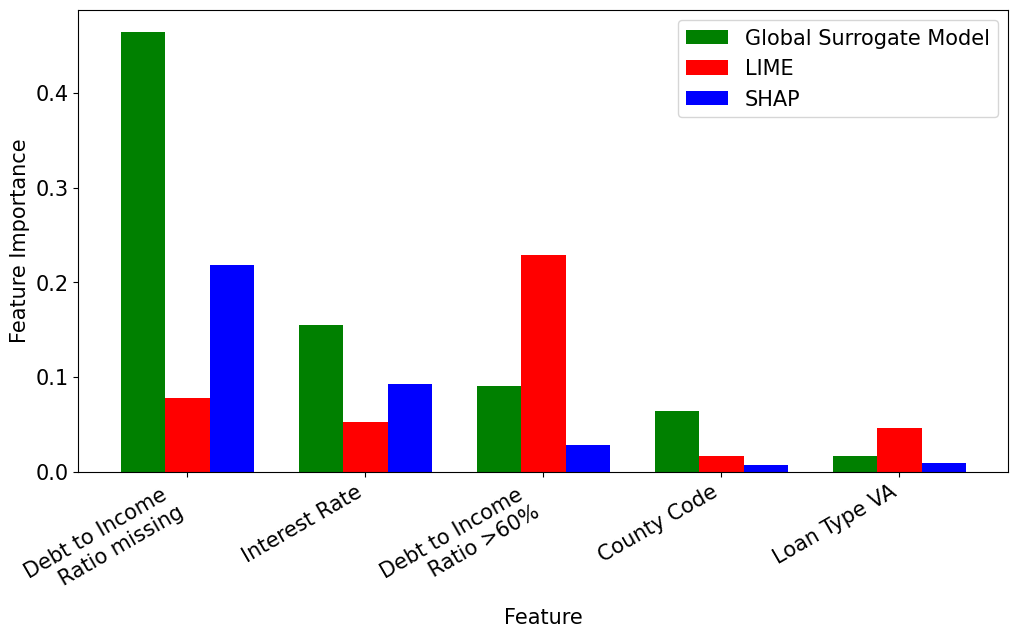
\includegraphics[width=0.85\textwidth]{images/CHXX_UPDATE_Surrogate_SHAP_LIME_combined.png}
    \caption{Global Surrogate Model compared to SHAP and LIME}
    \caption*{Analyzing the 5 most important features according to the global surrogate model implies that the overall trends of SHAP and LIME are close to the global explanations.}
    \label{fig:Global_Surrogate}
\end{figure}

\textbf{Performance}

Even without directly comparable benchmarks available (see \textbf{chapter \ref{subsec:Performance_Assessment}}), the initial model performance can be considered as good. Details can be found in \textbf{table \ref{tab:initial_model_performance_results_1}}.

\begin{table}[h]
    \centering
    \begin{tabular}{l c}
    \toprule
    \textbf{Metric} & \textbf{Value} \\
    \midrule
    \textbf{accuracy} & 0.90 \\
    \textbf{precision} & 0.88 \\
    \textbf{recall} & 0.96 \\
    \textbf{f1} & 0.92 \\
    \textbf{roc\_auc} & 0.94 \\
    \bottomrule
    \end{tabular}
    \caption{Metrics \#1: Initial Model}
    \caption*{The initial model shows a high accuracy and recall, but a lower precision and f1 score. The overall performance can be considered good.}
    \label{tab:initial_model_performance_results_1}
\end{table}

\textbf{Fairness}

\textbf{Table \ref{tab:initial_model_fairness_results_1}} shows the results of the fairness assessment of the initial model. The disparities in the true positive rate and false positive rate are relatively low, while the disparities in the true negative rate and false negative rate are higher.

\begin{table}[h]
    \caption{Metrics \#2: Initial Model}
    \begin{minipage}[t]{0.5\textwidth}
    \centering
    \begin{tabular}{lr}
    \toprule
    \textbf{Metric} & \textbf{Value} \\
    \midrule
    \textbf{Accuracy White} & 0.91 \\
    \textbf{Precision White} & 0.89 \\
    \textbf{Recall White} & 0.97 \\
    \textbf{F1 Score White} & 0.93 \\
    \textbf{AUC White} & 0.94 \\
    \textbf{Accuracy Black} & 0.89 \\
    \textbf{Precision Black} & 0.84 \\
    \textbf{Recall Black} & 0.92 \\
    \textbf{F1 Score Black} & 0.88 \\
    \textbf{AUC Black} & 0.95 \\
    \bottomrule
    \end{tabular}
    \end{minipage}\hfill
    \begin{minipage}[t]{0.5\textwidth}
    \centering
    \begin{tabular}{lr}
    \toprule
    \textbf{Metric} & \textbf{Value} \\
    \midrule
    \textbf{tpr\_disparity} & 0.95 \\
    \textbf{fpr\_disparity} & 0.77 \\
    \textbf{tnr\_disparity} & 1.05 \\
    \textbf{fnr\_disparity} & 2.51 \\
    \bottomrule
    \end{tabular}
    \end{minipage}
    \label{tab:initial_model_fairness_results_1}
    \caption*{The initial model shows a higher accuracy and recall for White applicants, but a higher precision and F1 score for Black applicants. The AUC is higher for Black applicants. The disparities in the true positive rate and false positive rate are relatively low, while the disparities in the true negative rate and false negative rate are higher.}
\end{table}

\subsection{Results of the Iterations}\label{subsec:Iterations}

None of the techniques applied in the iterations led to a significant increase in fairness. The \textit{reweighing} technique managed to improve the overall fairness of the model, but the other techniques did not manage to reach the same level of fairness. 
Figures \textbf{\ref{fig:Initial_Disparity}} to \textbf{\ref{fig:Calibrated_EqOdds_Disparity}} show that the disparity in loan grants between \textit{White} and \textit{Black or African American} applicants was not substantially reduced by any of the iterations, with the calibrated equalized odds algorithm even increasing the disparity.

\begin{figure}[h]
    \centering
    \begin{minipage}{0.5\textwidth}
        \centering
        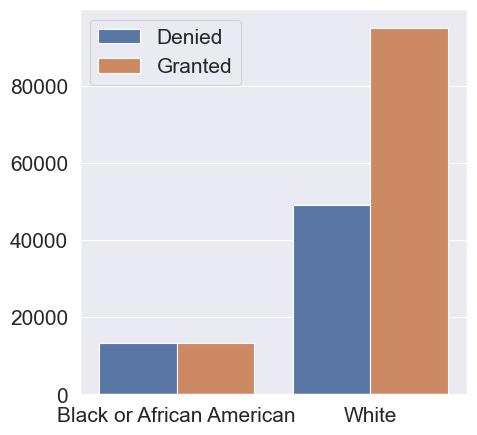
\includegraphics[width=\textwidth]{images/loan_grants_by_protected_attributes/initial.png}
        \caption{Initial Model Disparity}
        \label{fig:Initial_Disparity}
    \end{minipage}\hfill
    \begin{minipage}{0.5\textwidth}
        \centering
        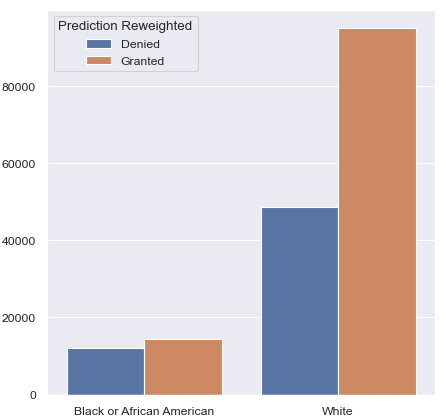
\includegraphics[width=\textwidth]{images/loan_grants_by_protected_attributes/reweighted.png}
        \caption{Reweighed Model Disparity}
        \label{fig:Reweighed_Disparity}
    \end{minipage}
    
    \vspace{1em} 
    
    \begin{minipage}{0.5\textwidth}
        \centering
        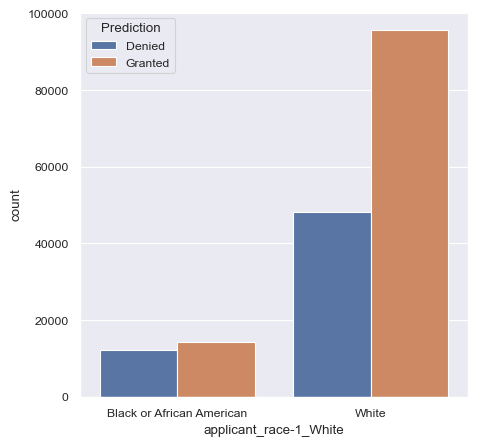
\includegraphics[width=\textwidth]{images/loan_grants_by_protected_attributes/correlation_removed.png}
        \caption{Corr. Rem. Model Disparity}
        \label{fig:Correlation_Removed_Disparity}
    \end{minipage}\hfill
    \begin{minipage}{0.5\textwidth}
        \centering
        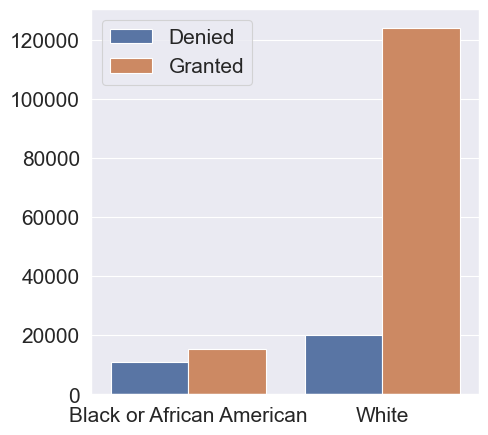
\includegraphics[width=\textwidth]{images/loan_grants_by_protected_attributes/calibrated_eqodds.png} 
        \caption{Cal. Eq. Odds Model Disparity}
        \label{fig:Calibrated_EqOdds_Disparity}
    \end{minipage}
    
    \label{fig:Racial_Disparities}
    \caption*{Apart from the Calibrated Equalized Odds model, which exhibits a higher amount of overall predicted grants, none of the iterations were able to substantially reduce the disparity in granted loans between races.}
\end{figure}

In terms of \textbf{performance}, the iterations did not lead to a significant increase in performance, with the \textit{Calibrated Equalized Odds} model even showing a significant decrease in performance. \textbf{Table \ref{tab:metrics_1_iterations}} shows the results of the performance assessment of the iterations.
All iterations tended to be closer to each other than expected. The best value (which is marked in bold), was only achieved at the third or fourth digit after the comma in many cases, leading to changes in the "best" model across different iterations.

\begin{table}[h]
    \centering
    \caption{Metrics \#1: Iterations}
    \begin{tabular}{l *{4}{>{$}c<{$}}}
    \toprule
    & \textbf{Initial Model} & \textbf{Reweighing} & \textbf{Calibrated Equalized Odds} & \textbf{Correlation Removal} \\
    \midrule
    \textbf{accuracy} & 0.90 & 0.90 & 0.73 & \textbf{0.91} \\
    \textbf{precision} & 0.88 & 0.88 & 0.69 & \textbf{0.88} \\
    \textbf{recall} & 0.96 & \textbf{0.97} & 0.97 & 0.97 \\
    \textbf{f1} & 0.92 & 0.92 & 0.81 & \textbf{0.92} \\
    \textbf{roc\_auc} & \textbf{0.94} & 0.94 & \text{NA} & \text{NA} \\
    \bottomrule
    \end{tabular}
    \caption*{Except the Calibrated Equalized Odds Model, all iterations show a similar performance to the initial model. The Correlation Removal Model shows a slightly higher accuracy and f1 score.}
    \label{tab:metrics_1_iterations}
\end{table}

Similarly to the performance, the iterations did not lead to a significant increase in (subgroup) fairness. The \textit{reweighing} technique managed to improve the overall fairness of the model, but the other techniques did not manage to reach the same level of fairness. \textbf{Table \ref{tab:metrics_2_1_iterations}} shows the results of the fairness assessment of the iterations for the first part of \textit{metrics \#2}.

\begin{table}[h]
    \centering
    \caption{Metrics \#2 (1): Iterations}
    \begin{tabular}{l *{4}{>{$}c<{$}}}
    \toprule
    & \textbf{Initial Model} & \textbf{Reweighing} & \textbf{Calibrated Equalized Odds} & \textbf{Correlation Removal} \\
    \midrule
    \textbf{Accuracy White} & 0.91 & 0.91 & 0.72 & \textbf{0.91} \\
    \textbf{Precision White} & \textbf{0.89} & 0.89 & 0.68 & 0.89 \\
    \textbf{Recall White} & 0.97 & 0.97 & \textbf{0.98} & 0.98 \\
    \textbf{F1 Score White} & 0.93 & 0.92 & 0.81 & \textbf{0.93} \\
    \textbf{AUC White} & \textbf{0.94} & 0.94 & \text{NA} & \text{NA} \\
    \midrule
    \textbf{Accuracy Black} & \textbf{0.89} & 0.88 & 0.81 & 0.88 \\
    \textbf{Precision Black} & 0.84 & 0.81 & 0.73 & \textbf{0.85} \\
    \textbf{Recall Black} & 0.92 & \textbf{0.97} & 0.93 & 0.92 \\
    \textbf{F1 Score Black} & 0.88 & \textbf{0.88} & 0.82 & 0.88 \\
    \textbf{AUC Black} & 0.95 & \textbf{0.95} & \text{NA} & \text{NA} \\
    \bottomrule
    \end{tabular}
    \caption*{Once again, the Calibrated Equalized Odds Model shows a significant decrease in performance. The other models show a similar performance to the initial model.}
    \label{tab:metrics_2_1_iterations}
\end{table}

In terms of disparities (see \textbf{table \ref{tab:metrics_2_2_iterations}}), the \textit{reweighing} technique managed to improve the overall fairness of the model, but the other techniques did not manage to reach the level of the initial model.
While across different model runs the disparities for the iterated models were very comparable, with the \textit{reweighing} technique consistently outperformung the other iterations, the performance in terms of disparities of the initial model varied strongly across different runs.

\begin{table}[h]
    \centering
    \caption{Metrics \#2 (2): Iterations}
    \begin{tabular}{l *{4}{>{$}c<{$}}}
    \toprule
    & \textbf{Initial Model} & \textbf{Reweighing} & \textbf{Calibrated Equalized Odds} & \textbf{Correlation Removal} \\
    \midrule
    \textbf{tpr\_disparity} & 0.95 & \textbf{1.00} & 0.95 & 0.94 \\
    \textbf{fpr\_disparity} & 0.77 & \textbf{1.00} & 0.43 & 0.76 \\
    \textbf{tnr\_disparity} & 1.01 & \textbf{1.00} & 2.23 & 1.06 \\
    \textbf{fnr\_disparity} & 2.51 & \textbf{0.84} & 3.25 & 3.42 \\
    \bottomrule
    \end{tabular}
    \caption*{In terms of disparities, the positive effects of reweighing show, with the algorithm outperforming the other iterations.}
    \label{tab:metrics_2_2_iterations}
\end{table}

Visualizing the results of the iterations in a comparison chart (\textbf{figure \ref{fig:Fairness_Comparison_Chart}}) shows that while the initial model managed to put out values with a comparably high fairness as measured by disparities, reweighing managed to improve this overall performance. The other two models however did not manage to reach the same level of fairness.

\begin{figure}
    \centering
    \caption{Fairness Comparison Chart}
    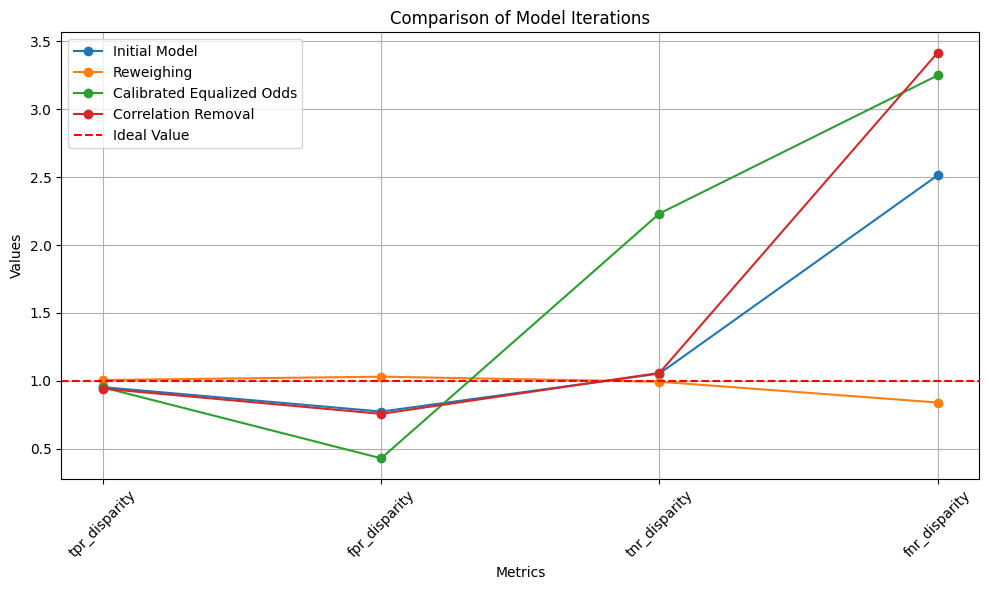
\includegraphics[width=0.85\textwidth]{images/CHXX_UPDATE_Results_Line.png}
    \caption*{While the initial model managed to put out values with a comparably high fairness as measured by disparities, reweighing managed to improve this overall performance. The other two models however did not manage to reach the same level of fairness.}
    \label{fig:Fairness_Comparison_Chart}
\end{figure}

% \section{Limitations}\label{sec:Limitations} - hier oder am Ende?

\section{Results}\label{sec:Results}

\subsection{Mortgage Classifier (Benchmark)}\label{subsec:Mortgage Classifier (Benchmark) Results}

In order to assess whether a predictive algorithm would pick up on and reproduce bias in the data, an initial classification model (as described in \textbf{chapter \ref{subsec:Model_Training_and_Prediction}} and detailed in \textbf{table \ref{tab:CH03_Model_Details}}) was trained on the HMDA dataset (see \textbf{chapter \ref{subsec:HMDA_Data}}) with the goal of predicting whether a mortgage would be granted or not for a given applicant.
The results of this model were assessed in terms of performance and fairness.

\textbf{Performance Assessment}

When fitting the neural network to the training data, the \textit{training accuracy} of the model improved rapidly initially, leveling off after a few epochs. The \textit{validation accuracy} started at a high level and constantly improved by small increments, suggesting that both the model learning process as well as the ability to generalize to previously unseen data were successful. 
The training process was stopped by an early\_stopping callback, with the ninth epoch being the one with the least validation loss. The training results of the best epoch were:
\begin{itemize}
    \item \textit{Training Accuracy}: 0.90
    \item \textit{Validation Accuracy}: 0.90
    \item \textit{Training Loss}: 0.28
    \item \textit{Validation Loss}: 0.28
\end{itemize}
The history of the training process is depicted in \textbf{figure \ref{fig:Model_Training_History}}.

\begin{figure}
    \centering
    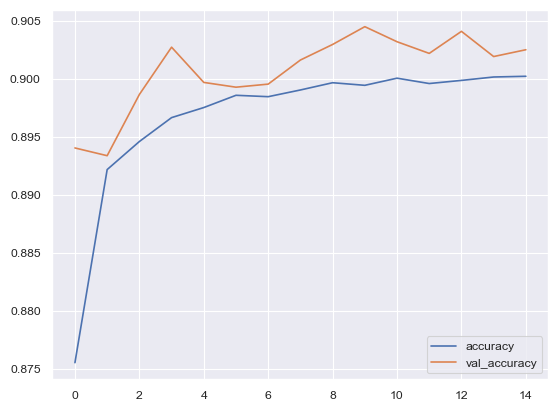
\includegraphics[width=0.85\textwidth]{images/Model_Training/Initial_Training_History.png}
    \caption{Training History of the Mortgage Classifier Model}
    \medskip
    \small
    The training history of the initial mortgage classifier model, showing the training and validation accuracy and loss over the course of the training process. The training accuracy improved constantly until the early\_stopping callback. The validation accuracy constantly improved, suggesting a successful learning process.
    \label{fig:Model_Training_History}
\end{figure}

The model was then evaluated on the test dataset, which was not seen by the model during training. The results of the performance evaluation (i.e. \textit{metrics \#1}) are shown in \textbf{table \ref{tab:Model_Evaluation}}. The model achieved an \textit{accuracy} of 0.90, a \textit{precision} of 0.88, a \textit{recall} of 0.97, and an \textit{F1-score} of 0.92. 
As stated in \textbf{chapter \ref{subsec:Model_Training_and_Prediction}}, the original model output were probabilities between 0 and 1. These could be used to calculate ROC AUC and plot the corresponding ROC curve, which can be seen in \textbf{figure \ref{fig:Model_Training_ROC}}. The \textit{ROC-AUC} score was 0.94, indicating a high level of model performance. 
Converting the probabilities into predictions with a threshold of 0.5 fulfilled the classification requirement. The \textit{confusion matrix} is depicted in \textbf{figure \ref{fig:Model_Confusion_Matrix}}. The model managed to achieve a high number of true positives and true negatives, while the number of false negatives was low. However, the number of false positives was nearly 8\% of all predictions.

\begin{table}[!htbp]
    \centering
    \begin{tabular}{l c}
    \toprule
    \textbf{Metric} & \textbf{Value} \\
    \midrule
    \textbf{accuracy} & 0.90 \\
    \textbf{precision} & 0.88 \\
    \textbf{recall} & 0.97 \\
    \textbf{f1} & 0.92 \\
    \bottomrule
    \end{tabular}
    \caption{Metrics \#1: Initial Model}
    \small
    The mortgage classifier model was evaluated on the test dataset, achieving an accuracy of 0.90, a precision of 0.88, a recall of 0.97, and an F1-score of 0.92.
    \label{tab:Model_Evaluation}
\end{table}

\begin{figure}
    \centering
    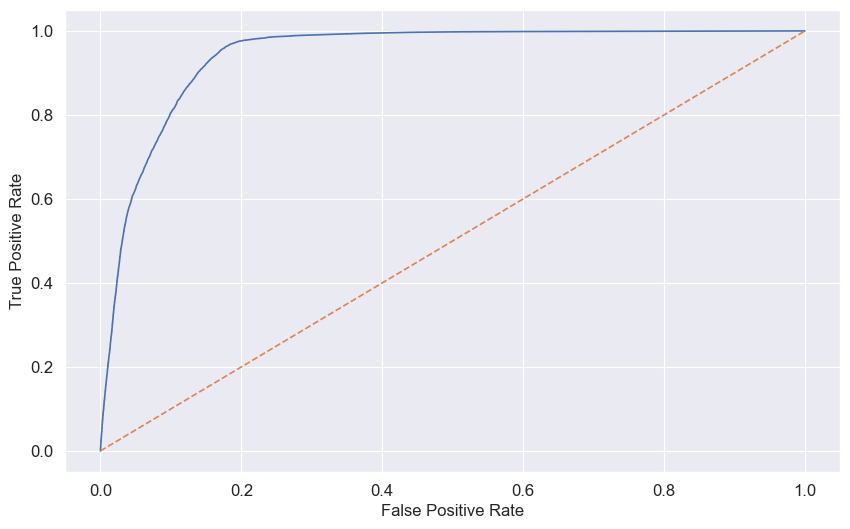
\includegraphics[width=0.85\textwidth]{images/Model_Training/Initial_ROC_curve.png}
    \caption{ROC curve of the Mortgage Classifier Model}
    \medskip
    \small
    The ROC curve is significantly above the diagonal baseline, indicating high predictive performance.
    \label{fig:Model_Training_ROC}
\end{figure}

\begin{figure}
    \centering
    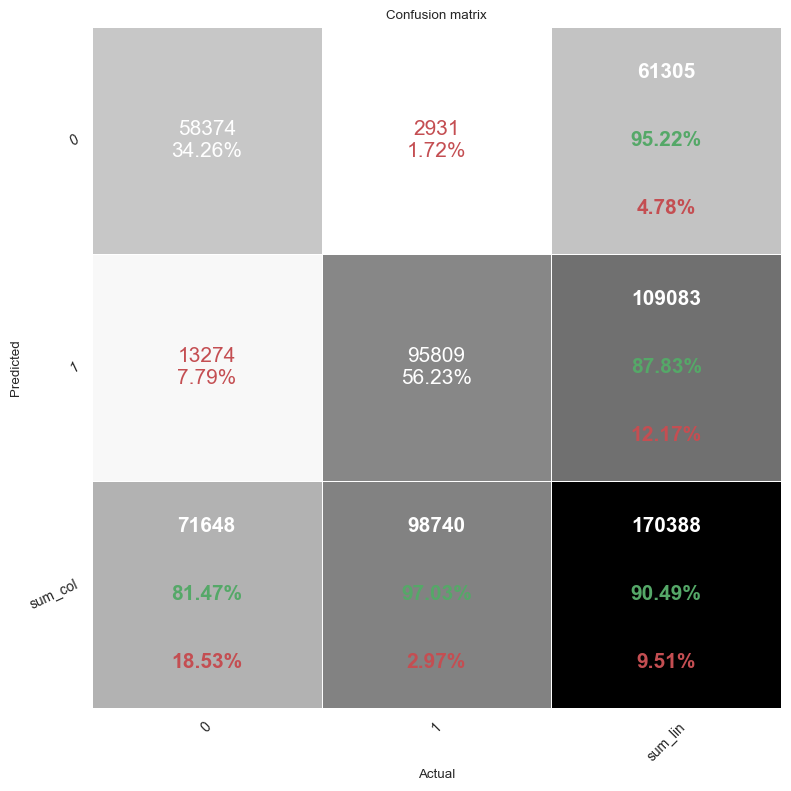
\includegraphics[width=0.85\textwidth]{images/Model_Training/Initial_Confusion_Matrix.png}
    \caption{Confusion Matrix on the Test Dataset of the Mortgage Classifier Model}
    \medskip
    \small
    The confusion matrix of the mortgage classifier model on the test dataset. The model achieved a high number of true positives and true negatives. The number of false negatives was low, however, false positives made up nearly 8\% of all predictions.
    \label{fig:Model_Confusion_Matrix}
\end{figure}

\textbf{Fairness Assessment}

Following the research question (see \textbf{chapter \ref{ch:Introduction}}), the \textit{detection of unfairness} in the predictions is an explicit goal of this thesis. To address this, the fairness assessment outlined in \textbf{chapter \ref{subsec:Model_Training_and_Prediction}} was applied to the predictions. The results of the fairness assessment (i.e. \textit{metrics \#2}) are shown in \textbf{table \ref{tab:Fairness_Assessment_Initial}}. 
The model performed slightly better for \textit{White} applicants than for \textit{Black} applicants. The \textit{accuracy} for \textit{White} applicants was 0.91, while it was 0.88 for \textit{Black} applicants. The \textit{precision} for \textit{White} applicants was 0.89, while it was 0.82 for \textit{Black} applicants. The \textit{recall} for \textit{White} applicants was 0.97, while it was 0.96 for \textit{Black} applicants. 
The \textit{F1-score} for \textit{White} applicants was 0.93, while it was 0.88 for \textit{Black} applicants. The \textit{AUC} for \textit{White} applicants was 0.94, while it was 0.95 for \textit{Black} applicants. 
In terms of disparities (where the optimal value is \textbf{1}), the model performed comparably well in all disciplines except the \textit{fnr\_disparity}, which was 1.42. This indicates that the model was more likely to predict a false negative for \textit{Black} applicants than for \textit{White} applicants.

\begin{table}[!htbp]
    \centering
    \begin{tabular}{lr}
    \toprule
    \textbf{Metric} & \textbf{Value} \\
    \midrule
    \textbf{Accuracy White} & 0.91 \\
    \textbf{Precision White} & 0.89 \\
    \textbf{Recall White} & 0.97 \\
    \textbf{F1 Score White} & 0.93 \\
    \textbf{AUC White} & 0.94 \\
    \midrule
    \textbf{Accuracy Black} & 0.88 \\
    \textbf{Precision Black} & 0.82 \\
    \textbf{Recall Black} & 0.96 \\
    \textbf{F1 Score Black} & 0.88 \\
    \textbf{AUC Black} & 0.95 \\
    \midrule
    \textbf{tpr\_disparity} & 0.99 \\
    \textbf{fpr\_disparity} & 0.96 \\
    \textbf{tnr\_disparity} & 1.01 \\
    \textbf{fnr\_disparity} & 1.42 \\
    \bottomrule
    \end{tabular}
    \caption{Metrics \#2: Initial Model}
    \label{tab:Fairness_Assessment_Initial}
    \small
    The benchmark model showed a slightly better performance for \textit{White} applicants than for \textit{Black} applicants. The disparities were comparably low, except for the \textit{fnr\_disparity}, which was 1.42.
\end{table}

\subsection{Explainability}\label{Explainability Results}

As stated in \textbf{chapter \ref{subsec:Explainability}}, three different approaches to explainability were utilized not only to support the analysis of fairness by providing insights into the model's decision-making process, but also to provide a better understanding of the model's behavior: \textit{SHAP}, \textit{LIME}, and a \textit{Global Surrogate Model}. 

\textbf{SHAP}

As stated in \textbf{chapter \ref{subsec:algorithms}}, the SHAP algorithm tries to game-theoretically distribute the value of the final prediction among the individual features considered.
\textbf{Figure \ref{fig:SHAP_beeswarm}} shows the SHAP beeswarm plot, which displays the distribution of the SHAP values for each feature in the dataset. The color indicates the feature value (red = higher; blue = lower), while the x-axis shows the SHAP value (left of center = negative; right of center = positive). The y-axis shows the feature name. The plot includes 150 values from the SHAP values of the test dataset.
It showed that the most influential features according to SHAP were \textit{debt\_to\_income\_ratio\_missing, interest\_rate, loan\_to\_value\_ratio}, and \textit{debt\_to\_income\_ratio\_>60\%}.
While it was apparent how missingness in the debt to income ratio (missingness is negative, availability is positive) and values >60\% in the debt to income ratio (higher is negative, lower is positive) affected the model decision, interest rates and the loan-to-value-ratios as the numerical variables were less intuitive to interpret.
Although most medium to high interest rates seemed to be related with slight negative impacts, there also was a cluster of higher values for these variables corresponding with positive prediction influences.
As all other variables were categorical, their interpretations were straightforward. Albeit their absolute impact in terms of SHAP values was limited, it is noteworthy that the \textit{protected variables} of race and sex were in fact picked up on by the model.
In every case where a decision was negatively influenced by the \textit{race} of the applicant, the applicant in question was Black or African American (as can be inferred from all values left of the center of the x-axis for \textit{applicant\_race-1\_White} being colored blue for this feature, meaning a lower value, which in turn means Black or African American ethnicity).
A similar picture was observed for the \textit{sex} of the applicant: In most cases where the model picked up on the sex being an influential factor on the model decision, the applicant in question was \textit{female} and vice versa.

\begin{figure}[!htbp]
    \centering
    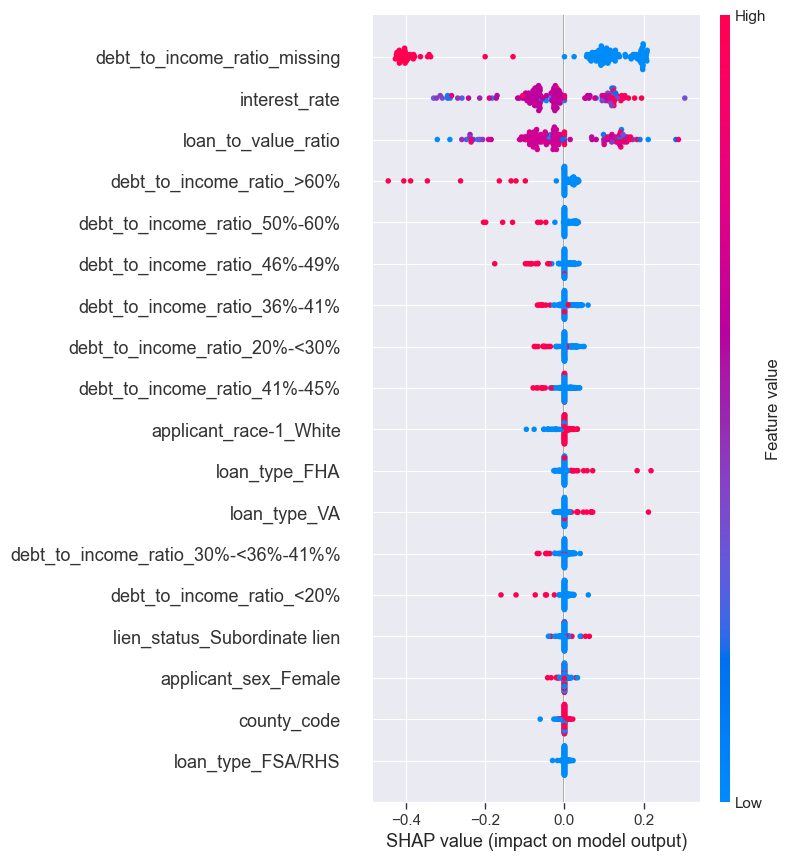
\includegraphics[width=0.85\textwidth]{images/SHAP_Individual_Analyses/beeswarm.png}
    \caption{SHAP beeswarm plot}
    \medskip
    \small
    The SHAP beeswarm plot shows the distribution of the SHAP values for each feature in the dataset. The color indicates the feature value, while the x-axis shows the SHAP value. The y-axis shows the feature name.
    \label{fig:SHAP_beeswarm}
\end{figure}

The \textit{expected value} of the SHAP values (i.e. the baseline before consideration of any feature importance) was \textit{0.57}. This corresponds to the imbalance in the original HMDA data (see \textbf{chapter \ref{fig:CHXX_Target_Variable_Distribution}}).
\textbf{Figure \ref{fig:SHAP_Individual_Analyses}} shows the SHAP values for four selected applicants. The force plots displayed show how the individual values of the features influence the model's decision according to SHAP. 
Each individual prediction results from the aforementioned \textit{expected value} and the sum of inferred importances of the features (exemplarily, in the first plot displayed in \textbf{figure \ref{fig:SHAP_Individual_Analyses}}, the feature importances amount to roughly positive 0.4, leading to a total value of 0.97 and therefore a positive prediction, i.e. a granted mortgage).
It shows that SHAP attributes a high importance to (missingness of) the Debt to income ratio. Due to the values being scaled, a value of \textit{-0.59} corresponds to \textit{debt\_to\_income\_ratio\_missing == False} and a value of \textit{1.68} corresponds to \textit{debt\_to\_income\_ratio\_missing == True}. Therefore, SHAP considers missingness in this variable as negative and availability as positive.
Considering the last applicant displayed (\textit{Black or African American Male, Debt to Income Ratio available}), it does however show that even availabilty of the Debt to Income Ratio does not guarantee a positive model decision.
According to SHAP, none of the decisions displayed here (and in the whole set of predictions in general) were significantly informed by any protected attribute. However, confounding factors might still be present, as the model might have learned to discriminate based on other features that are correlated with the protected attributes.

\begin{figure}[!htbp]
    \centering
    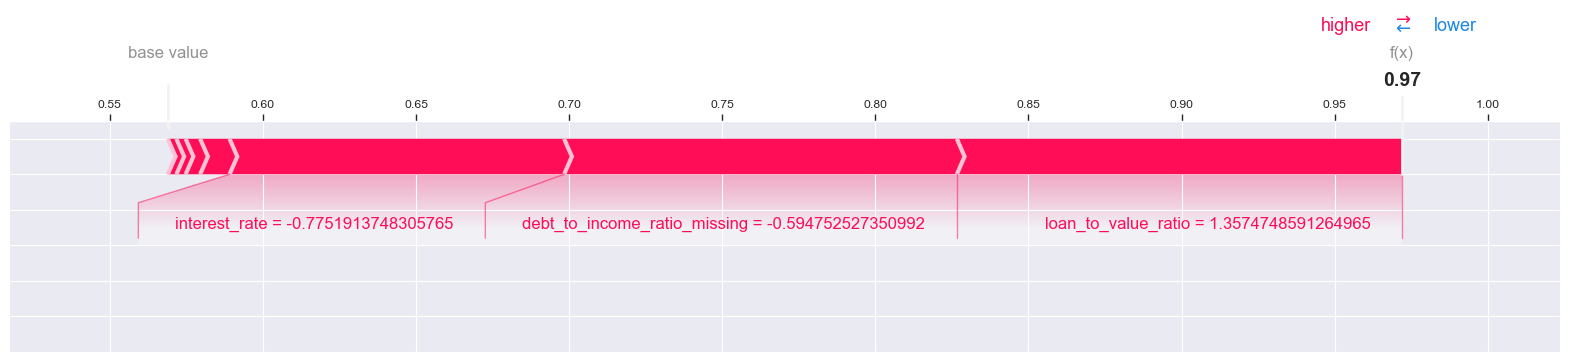
\includegraphics[width=0.95\textwidth]{images/SHAP_Individual_Analyses/SHAP_individual_0.png}
    \small
    White Male, Debt to Income Ratio available
    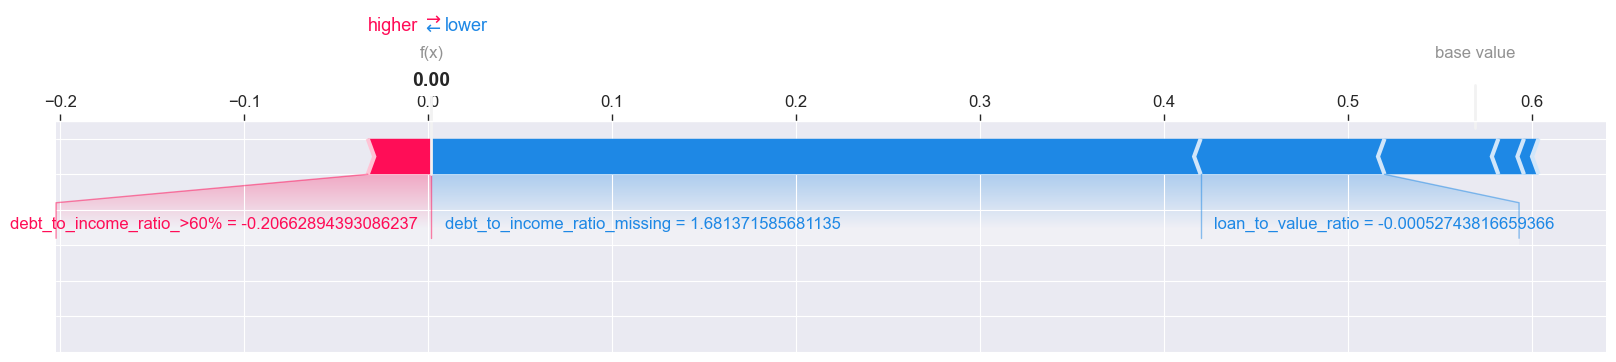
\includegraphics[width=0.95\textwidth]{images/SHAP_Individual_Analyses/SHAP_individual_1.png}
    \small
    White Male, Debt to Income Ratio missing
    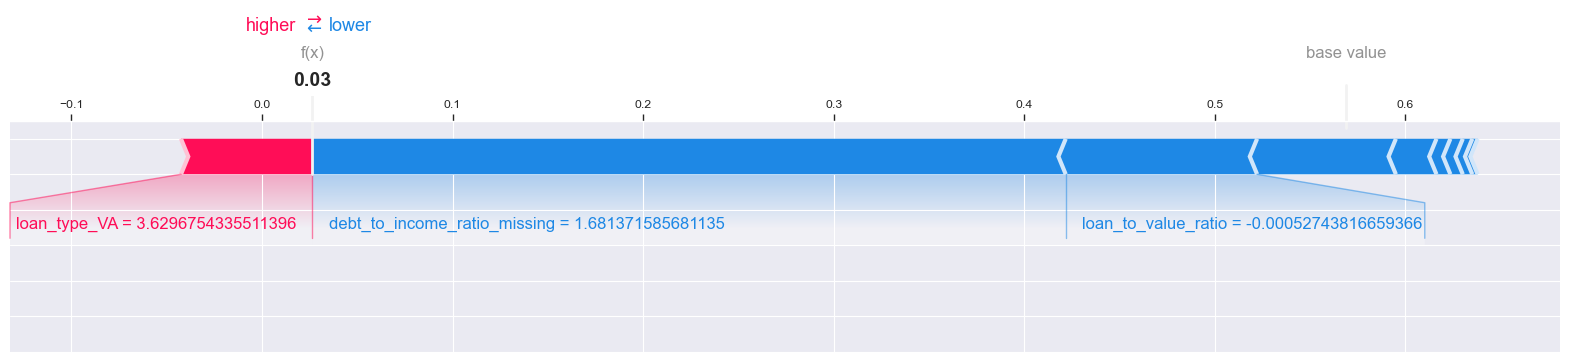
\includegraphics[width=0.95\textwidth]{images/SHAP_Individual_Analyses/SHAP_individual_21.png}
    \small
    Black or African American Male, Debt to Income Ratio missing
    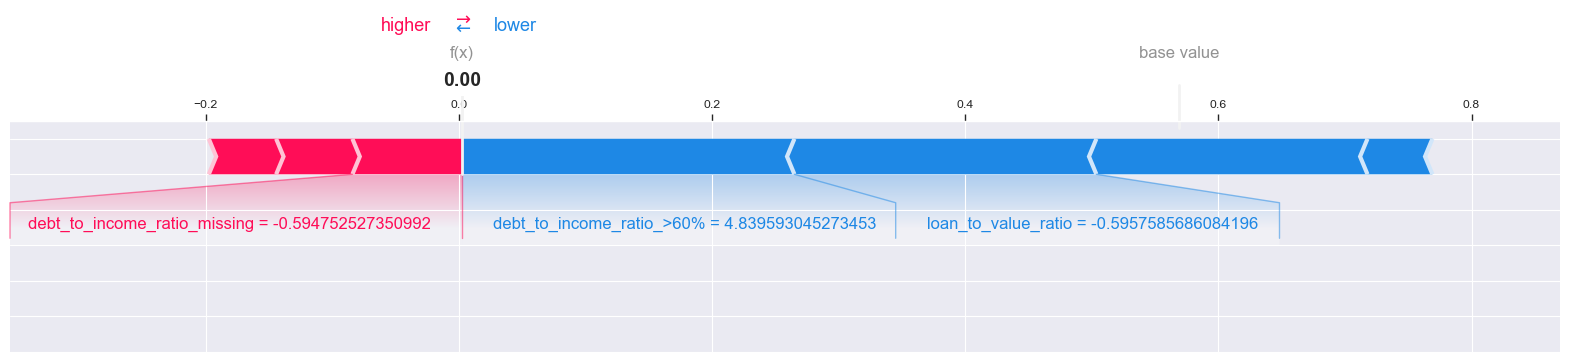
\includegraphics[width=0.95\textwidth]{images/SHAP_Individual_Analyses/SHAP_individual_139.png}
    \small
    Black or African American Male, Debt to Income Ratio available
    \caption{Selected SHAP Individual Analyses}
    \medskip
    \small
    Comparing four selected Male applicants with different characteristics shows that, in general, SHAP attributes a high importance to (missingness of) the Debt to Income Ratio. However, it is not the sole decision criterion, as the last applicant displayed shows.
    \label{fig:SHAP_Individual_Analyses}
\end{figure}

\textbf{LIME}

The LIME algorithm, in contrast to SHAP, tries to explain the model's decision on a local level by approximating the model's behavior around a single prediction (see \textbf{chapter \ref{subsec:algorithms}}).
\textbf{Figure \ref{fig:LIME_Individual_Analyses}} shows the LIME individual feature importance plot for a selected applicant, specifically the same applicant that is denoted as \textit{White Male, Debt to Income Ratio available} in \textbf{figure \ref{fig:SHAP_Individual_Analyses}}. The x-axis shows the feature importance, while the y-axis shows the feature name.
It showed that LIME attributes a high importance to the \textit{loan type} and the \textit{debt to income ratio}. Once again, the \textit{protected attributes} had very little absolute influence on the model's decision according to LIME.

\begin{figure}[!htbp]
    \centering
    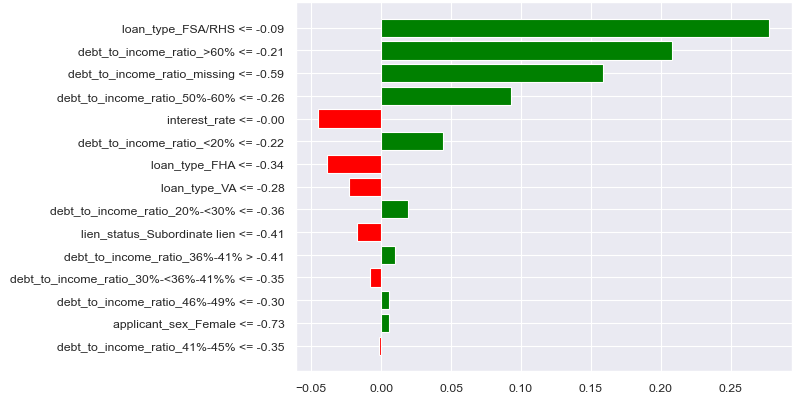
\includegraphics[width=0.85\textwidth]{images/CHXX_LIME_individual.png}
    \caption{LIME Individual Feature Importance}
    \medskip
    \small
    The LIME individual feature importance plot shows the direction and the impact of the features on the model's decision for a selected applicant. The x-axis shows the feature importance, while the y-axis shows the feature name.
    \label{fig:LIME_Individual_Analyses}
\end{figure}

While the overall explanations on which features are influential are similar for both SHAP and LIME, the actual impact of the features varies significantly. While this is not a direct threat to the quality of the results of this thesis, it is a reminder that explainability algorithms need to be analyzed carefully. 
This ties with the findings of Krishna et al. \parencite{Krishna2022}, who emphasize the importance of understanding the underlying assumptions of explainability algorithms and the need for a more comprehensive evaluation of their results.

\textbf{Global Surrogate Model}

To validate the results of the local explanations, a \textit{Global Surrogate Model} was used. \textbf{figure \ref{fig:Global_Surrogate}} shows the results of the global surrogate model. Specifically, the five most important features according to the global surrogate model are compared to the SHAP and LIME explanations in terms of their relative performance.
It showed that all three explanation algorithms mainly agree on the three most important features in the data (\textit{debt\_to\_income\_ratio\_missing, interest\_rate}, and \textit{debt\_to\_income\_ratio\_>60\%}), although LIME attributes a different order of importance to them compared to SHAP and the global surrogate model.

\begin{figure}[!htbp]
    \centering
    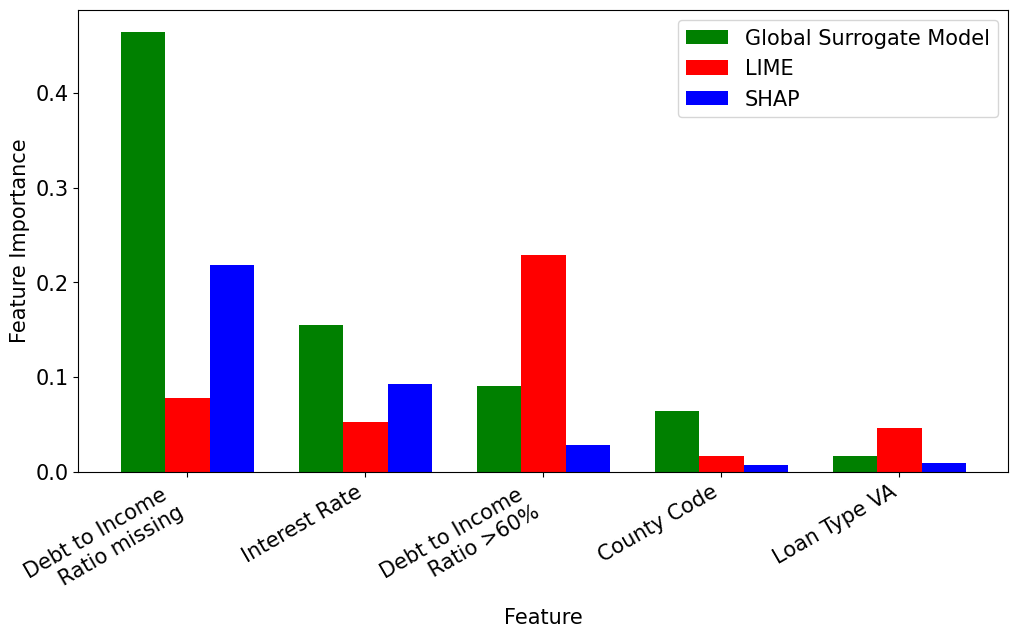
\includegraphics[width=0.85\textwidth]{images/CHXX_UPDATE_Surrogate_SHAP_LIME_combined.png}
    \caption{Global Surrogate Model compared to SHAP and LIME}
    \medskip
    \small
    Analyzing the 5 most important features according to the global surrogate model implies that the overall trends of SHAP and LIME are close to the global explanations.
    \label{fig:Global_Surrogate}
\end{figure}

\subsection{Fairness Adjustments}\label{Fairness Adjustments Results}

While the performance of the benchmark mortgage classifier detailed in \textbf{chapter \ref{subsec:Mortgage Classifier (Benchmark) Results}} was satisfactory, the scope of this thesis (see \textbf{chapter \ref{ch:Introduction}}) included taking an iterative approach to improve fairness without sacrificing predictive performance, as outlined in \textbf{chapter \ref{subsec:Iterations}}.
To this end, the following fairness adjustments were applied to the model: \textit{Reweighing}, \textit{Correlation Remover} and \textit{Calibrated Equalized Odds}. The aim was to reach improvement in at least one of the two metric sets, compared to the benchmark performance depicted in \textbf{table \ref{tab:Model_Evaluation}} (\textit{metrics \#1}) and \textbf{table \ref{tab:Fairness_Assessment_Initial}} (\textit{metrics \#2}).

\textbf{Reweighing}

XXX

\textbf{Correlation Remover}

XXX

\textbf{Calibrated Equalized Odds}

XXX

\textbf{Summary}

Considering the overall \textit{performance} of the different approaches, all models except the \textit{calibrated equalized odds} algorithms performed on a similar, good level (see \textbf{table \ref{tab:metrics_1_iterations_summary}}).
The \textit{correlation removal} algorithm managed to slightly outperform the benchmark model in terms of \textit{accuracy}, \textit{precision}, and \textit{f1-score}, while the \textit{calibrated equalized odds} algorithm managed to slightly outperform the benchmark model in terms of \textit{recall}.

\begin{table}[!htbp]
    \centering
    \begin{tabular}{l *{4}{>{$}c<{$}}}
    \toprule
    & \textbf{Initial Model} & \textbf{Reweighing} & \textbf{Calibrated Equalized Odds} & \textbf{Correlation Removal} \\
    \midrule
    \textbf{accuracy} & 0.90 & 0.90 & 0.73 & \textbf{0.91} \\
    \textbf{precision} & 0.88 & 0.88 & 0.69 & \textbf{0.88} \\
    \textbf{recall} & 0.97 & 0.97 & \textbf{0.97} & 0.97 \\
    \textbf{f1} & 0.92 & 0.92 & 0.81 & \textbf{0.92} \\
    \textbf{roc\_auc} & \textbf{0.94} & 0.94 & \text{NA} & \text{NA} \\
    \bottomrule
    \end{tabular}
    \caption{Metrics \#1: Fairness Adjustments Summary}
    \small
    Results of \textit{metrics \#1} for all applied algorithms. The values are rounded, the highest scores are marked \textbf{bold}.
    \label{tab:metrics_1_iterations_summary}
\end{table}

In terms of \textit{fairness}, no significant optimizations could be achieved. The \textit{reweighing} technique managed to improve the overall fairness of the model, but the other techniques did not manage to reach the same level of fairness. 
\textbf{Figure \ref{fig:Bar_Grant_per_Race}} shows that the differences in loan grants between \textit{White} and \textit{Black or African American} applicants was not substantially reduced by any of the iterations, with the calibrated equalized odds algorithm even increasing the difference.

\begin{figure}[!htbp]
    \centering
    \begin{minipage}{0.5\textwidth}
        \centering
        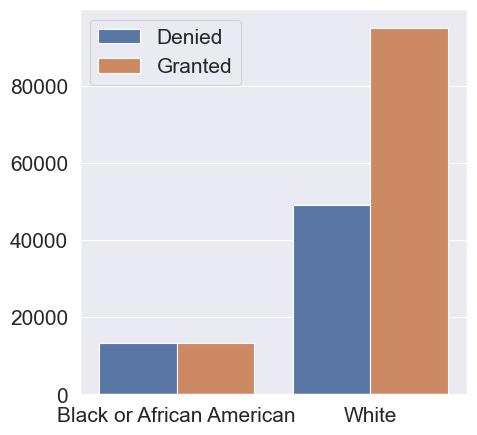
\includegraphics[width=\textwidth]{images/loan_grants_by_protected_attributes/initial.png}
        \small
        Benchmark Model
    \end{minipage}\hfill
    \begin{minipage}{0.5\textwidth}
        \centering
        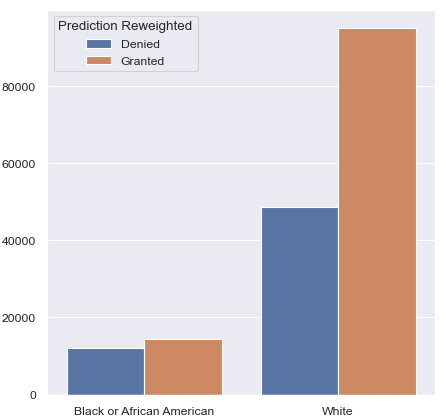
\includegraphics[width=\textwidth]{images/loan_grants_by_protected_attributes/reweighted.png}
        \small
        Reweighing
    \end{minipage}
    
    \begin{minipage}{0.5\textwidth}
        \centering
        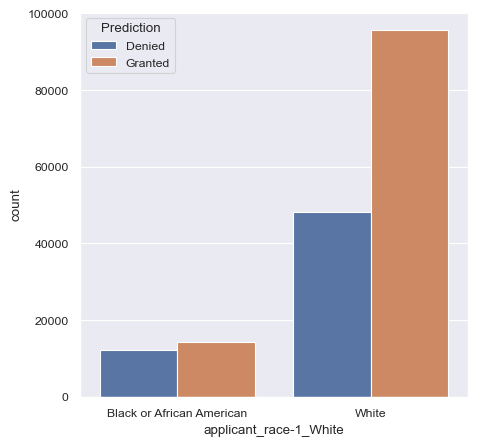
\includegraphics[width=\textwidth]{images/loan_grants_by_protected_attributes/correlation_removed.png}
        \small
        Correlation Removal
    \end{minipage}\hfill
    \begin{minipage}{0.5\textwidth}
        \centering
        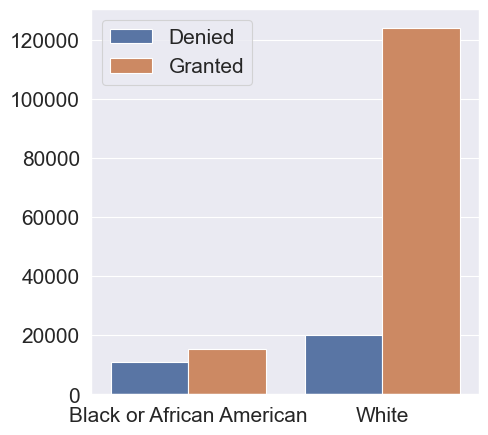
\includegraphics[width=\textwidth]{images/loan_grants_by_protected_attributes/calibrated_eqodds.png} 
        \small
        Calibrated Equalized Odds
    \end{minipage}
    
    \caption{Differences in Positive Predictions per Model}
    \label{fig:Bar_Grant_per_Race}
    \medskip
    \small
    Apart from the Calibrated Equalized Odds model, which exhibits a higher amount of overall predicted grants, none of the iterations were able to substantially reduce the disparity in granted loans between races.
\end{figure}

\textbf{Figure \ref{fig:Fairness_Adjustments_Results_Line}} shows the results of the fairness adjustments in terms of the \textit{disparities} of the model. The disparities were calculated for the \textit{true positive rate}, the \textit{false positive rate}, the \textit{true negative rate}, and the \textit{false negative rate}. 
The disparities were calculated for the \textit{White} and \textit{Black or African American} applicants. As they are relative terms, only the relation of the disparities to the other group is shown.
The disparities were comparably low for the \textit{true positive rate}, while all the other disparities show at least one outlier. The \textit{reweighed} model was the only one that produces satisfactory results in terms of fairness as measured by disparities across all four KPIs, with the benchmark model coming in second.

\begin{figure}[!htbp]
    \centering
    \includegraphics[width=0.85\textwidth]{images/CHXX_Update_Results_Line.png}
    \caption{Fairness Adjustments Results}
    \medskip
    \small
    The results of the fairness adjustments in terms of the disparities of the model. The disparities were calculated for the \textit{true positive rate}, the \textit{false positive rate}, the \textit{true negative rate}, and the \textit{false negative rate}. They were calculated for the \textit{White} and \textit{Black or African American applicants}. Values closer to 1 are better, the gray area represents a good level of fairness.
    \label{fig:Fairness_Adjustments_Results_Line}
\end{figure}

Adding up all fairness metrics for all iterations (see \textbf{table \ref{tab:metrics_2_iterations_summary}}) resulted in a mixed picture.
While the \textit{reweighing} algorithm managed to improve the fairness of the outcomes in terms of disparities (as can also be inferred from \textbf{figure \ref{fig:Fairness_Adjustments_Results_Line}}), the predictive power of the model for subgroups did not show a single optimal model.

\begin{table}[!htbp]
    \centering
    \begin{tabular}{l *{4}{>{$}c<{$}}}
    \toprule
    & \textbf{Initial Model} & \textbf{Reweighing} & \textbf{Calibrated Equalized Odds} & \textbf{Correlation Removal} \\
    \midrule
    \textbf{Accuracy White} & 0.91 & 0.91 & 0.72 & \textbf{0.91} \\
    \textbf{Precision White} & \textbf{0.89} & 0.89 & 0.68 & 0.89 \\
    \textbf{Recall White} & 0.97 & 0.97 & \textbf{0.98} & 0.98 \\
    \textbf{F1 Score White} & 0.93 & 0.93 & 0.81 & \textbf{0.93} \\
    \textbf{AUC White} & \textbf{0.94} & 0.94 & \text{NA} & \text{NA} \\
    \midrule
    \textbf{Accuracy Black} & 0.88 & 0.88 & 0.81 & \textbf{0.89} \\
    \textbf{Precision Black} & 0.82 & 0.81 & 0.73 & \textbf{0.84} \\
    \textbf{Recall Black} & 0.96 & \textbf{0.97} & 0.93 & 0.93 \\
    \textbf{F1 Score Black} & 0.88 & \textbf{0.88} & 0.82 & 0.88 \\
    \textbf{AUC Black} & \textbf{0.95} & 0.95 & \text{NA} & \text{NA} \\
    \midrule
    \textbf{tpr\_disparity} & 0.99 & \textbf{0.99} & 0.95 & 0.96 \\
    \textbf{fpr\_disparity} & 0.96 & \textbf{1.00} & 0.43 & 0.80 \\
    \textbf{tnr\_disparity} & 1.01 & \textbf{1.00} & 2.23 & 1.05 \\
    \textbf{fnr\_disparity} & 1.42 & \textbf{1.20} & 3.25 & 2.67 \\
    \bottomrule
    \end{tabular}
    \caption{Metrics \#2: Fairness Adjustments Summary}
    \small
    Results of \textit{metrics \#2} for all applied algorithms. The values are rounded, the highest scores (respectively those closest to 1 for the disparity calculations) are marked \textbf{bold}.
    \label{tab:metrics_2_iterations_summary}
\end{table}

% appendix

\printbibliography

\end{document}